C++不提供开箱即用的图形用户界面(GUI)编程。首先,我们应该理解GUI与特定的操作系统(OS)紧密相连。可以在Windows中使用Windows API编写GUI应用程序,也可以在Linux中使用特定于Linux的API编写GUI应用程序等。每个操作系统都有自己特定形式的Windows和GUI组件。 \par
我们在第1章中讨论了不同的平台及其差异。当讨论GUI编程时,平台之间的差异更加令人生畏。跨平台开发已经成为GUI开发人员生活中的一大难题。他们必须专注于特定的操作系统。为其他平台实现相同的应用程序再次花费了几乎相同的工作量。这是对时间和资源的巨大浪费。Java等语言提供了在虚拟环境中运行应用程序的智能模型。这允许开发人员专注于一种语言和一个项目,因为环境负责在不同平台上运行应用程序。这种方法的一个主要缺点是强迫用户安装虚拟机,并且与特定于平台的应用程序相比,执行时间较慢。 \par
为了解决这些问题,创建了Qt框架。在本章中,我们将了解Qt框架如何支持跨平台GUI应用程序开发。要做到这一点,您需要熟悉Qt及其关键特性。这将允许您使用您最喜欢的编程语言——C++开发GUI应用程序。我们将从理解Qt的GUI开发方法开始,然后我们将涵盖它的概念和特性,如信号和槽,以及模型/视图编程。 \par

本章中,我们将了解以下内容: \par

\begin{itemize}
	\item 跨平台GUI编程基础
	\item Qt核心组件
	\item 使用Qt widget
	\item 用Qt网络设计一个网络应用程序
\end{itemize}

\noindent\textbf{}\ \par
\textbf{编译器要求} \ \par
您将需要安装最新的Qt框架来运行本章中的示例。我们建议使用Qt Creator作为你的项目的IDE。要下载Qt以及相应的工具,请访问Qt .io网站并选择该框架的开源版本。。可以从这里获取本章的源码文件:https:/​/github.​com/PacktPublishing/Expert-CPP \par

\noindent\textbf{}\ \par
\textbf{理解跨平台GUI编程} \ \par
每个操作系统都有自己的API,并与GUI有关。当公司计划设计、实现和发布桌面应用程序时,他们应该决定关注哪个平台。在一个平台上工作的开发团队需要花费几乎相同的时间为另一个平台编写相同的应用程序。最大的原因是OS提供了不同的方法和API,API的复杂性也可能在及时实现应用程序方面扮演重要角色。例如,官方文档中的以下代码片段展示了如何在Windows中使用C++创建按钮: \par

\begin{lstlisting}[caption={}]
HWND hwndButton = CreateWindow(
	L"BUTTON", // Predefined class; Unicode assumed
	L"OK", // Button text
	WS_TABSTOP | WS_VISIBLE | WS_CHILD | BS_DEFPUSHBUTTON, // Styles
	10, // x position
	10, // y position
	100, // Button width
	100, // Button height
	m_hwnd, // Parent window
	NULL, // No menu.
	(HINSTANCE)GetWindowLong(m_hwnd, GWL_HINSTANCE),
	NULL); // Pointer not needed.
\end{lstlisting}

处理Windows GUI编程需要你使用HWND、HINSTACNCE和许多其他命名怪异、令人困惑的组件。 \par
.NET框架对Windows GUI编程进行了重大改进。如果你想要支持Windows以外的操作系统,在使用.NET框架之前,必须三思而后行。 \par
然而,为了支持多个操作系统,仍然需要深入研究API来实现相同的应用程序,以覆盖所有的操作系统用户。下面的代码展示了在Linux中使用Gtk+GUI工具包创建按钮的示例: \par

\begin{lstlisting}[caption={}]
GtkWidget* button = gtk_button_new_with_label("Linux button");
\end{lstlisting}

与Windows API相比,它似乎更容易理解。但是,您应该深入研究带有Gtk前缀的GtkWidgets和其他组件,以了解有关它们的更多信息。 \par
正如我们已经提到的,跨平台语言,如Java和.Net Core使用虚拟机在不同的平台上运行代码。Qt框架使用基于平台的编译方法支持跨平台GUI编程。让我们就C++语言来讨论这两种方式吧。 \par

\noindent\textbf{}\ \par
\textbf{如Java一样使用C++} \ \par
像Java或C\#这样的语言有不同的编译模型。本书第一章介绍了C++的编译模型。首先,我们认为C++是一种完全可编译的语言,而Java是一种混合模型语言。它将源代码编译为称为\textbf{字节码}的中间表示,然后虚拟机通过将其转换为特定平台的机器码来运行它。 \par
下图描述了C++和Java编译模型之间的区别: \par

\begin{center}
	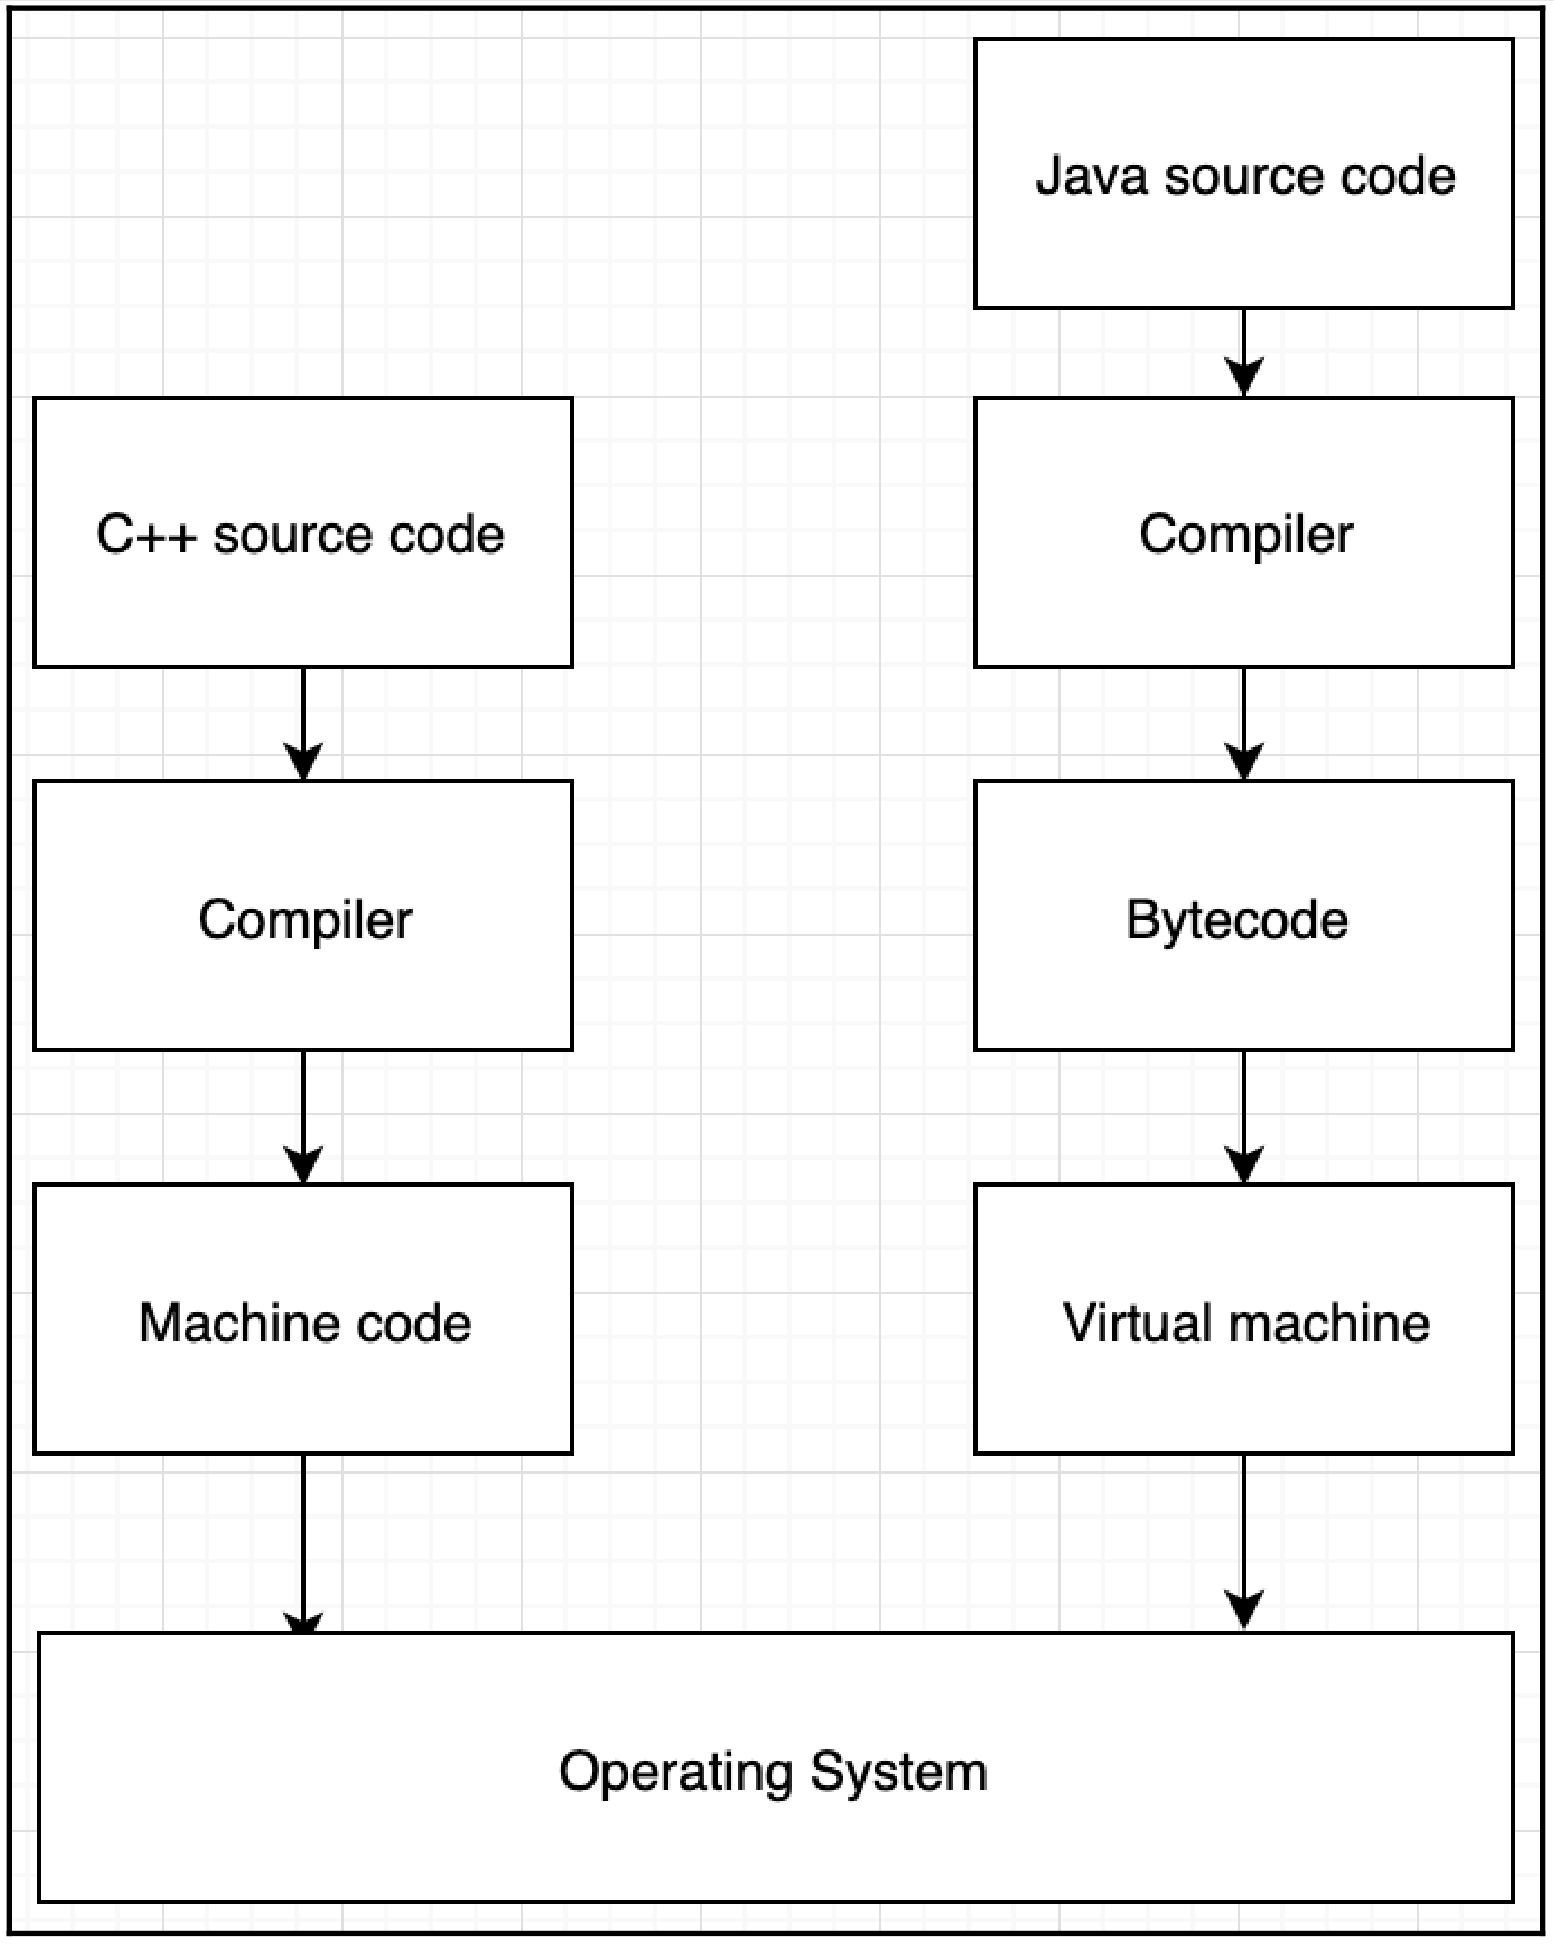
\includegraphics[width=0.8\textwidth]{content/Section-2/Chapter-14/1}
\end{center}

Java虚拟机(JVM)充当中间层,对每个平台都有一个独特的实现。用户需要在运行Java程序之前安装虚拟机的特定实现,安装过程只发生一次。另一方面,C++程序被翻译成机器码,这些机器码在没有JVM等中间层环境的情况下运行。这就是为什么C++应用程序通常更快的原因之一。当我们在某个平台上编译C++程序时,编译器输出一个可执行文件,该文件由特定于该平台的格式的指令组成。当我们将应用程序转移到另一个平台时,它就无法运行了。 \par
另一个平台不能识别它的格式,也不能识别它的指令(尽管它们在某些方面可能相似)。Java方法的工作原理是提供一些字节码,这些字节码对于虚拟机的所有实现都是相同的。但是虚拟机知道它们为作为输入的字节码生成什么指令。相同的字节码可以在许多安装了虚拟机的计算机上运行。下面的图表演示了Java应用程序编译模型: \par

\begin{center}
	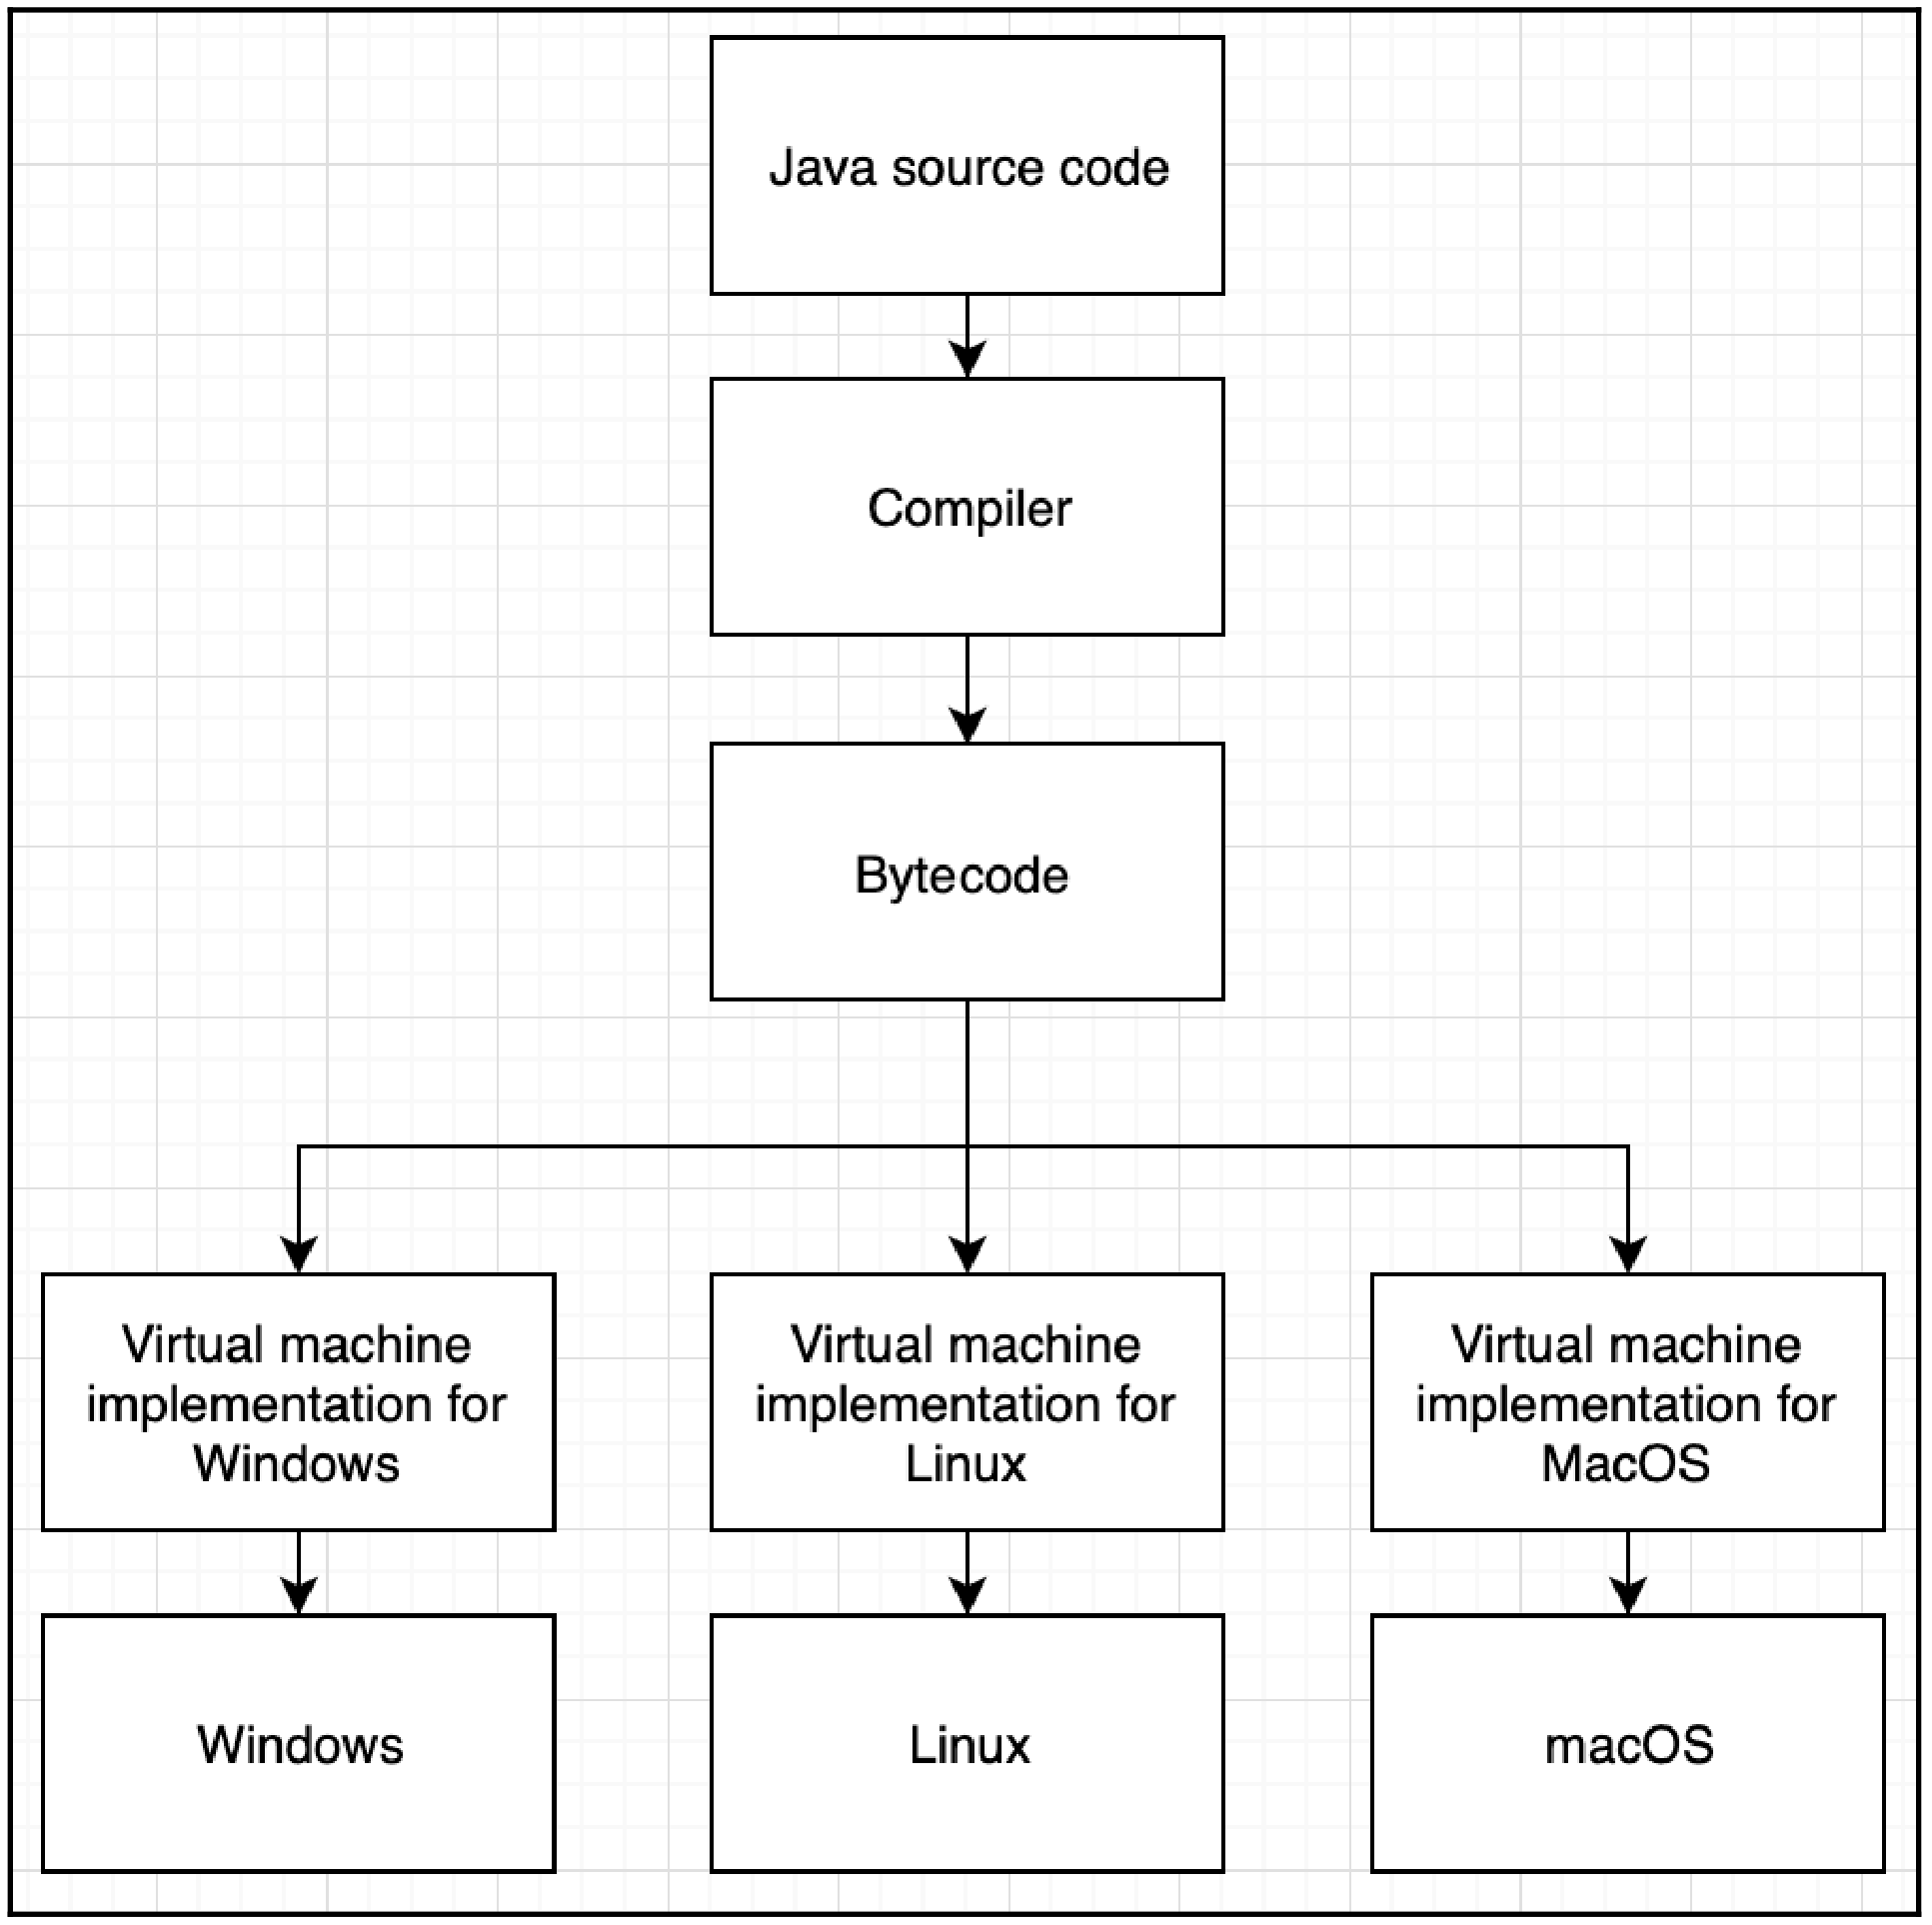
\includegraphics[width=1.0\textwidth]{content/Section-2/Chapter-14/2}
\end{center}

源代码编译成可以在每个操作系统上运行的字节码。但是,必须为每个操作系统提供自己的虚拟机实现。这意味着我们可以在任何操作系统上运行Java应用程序,只要我们安装了专门为该操作系统实现的JVM。 \par
尽管C++是一种跨平台语言,这意味着我们不需要修改代码来在其他平台上编译它,但这种语言并不支持GUI编程。如前所述,要编写GUI应用程序,我们需要直接从代码访问OS API。这使得C++ GUI应用程序依赖于平台,因为您需要修改代码库以在另一个平台上编译它。下图显示了GUI如何破坏了语言的跨平台特性: \par

\begin{center}
	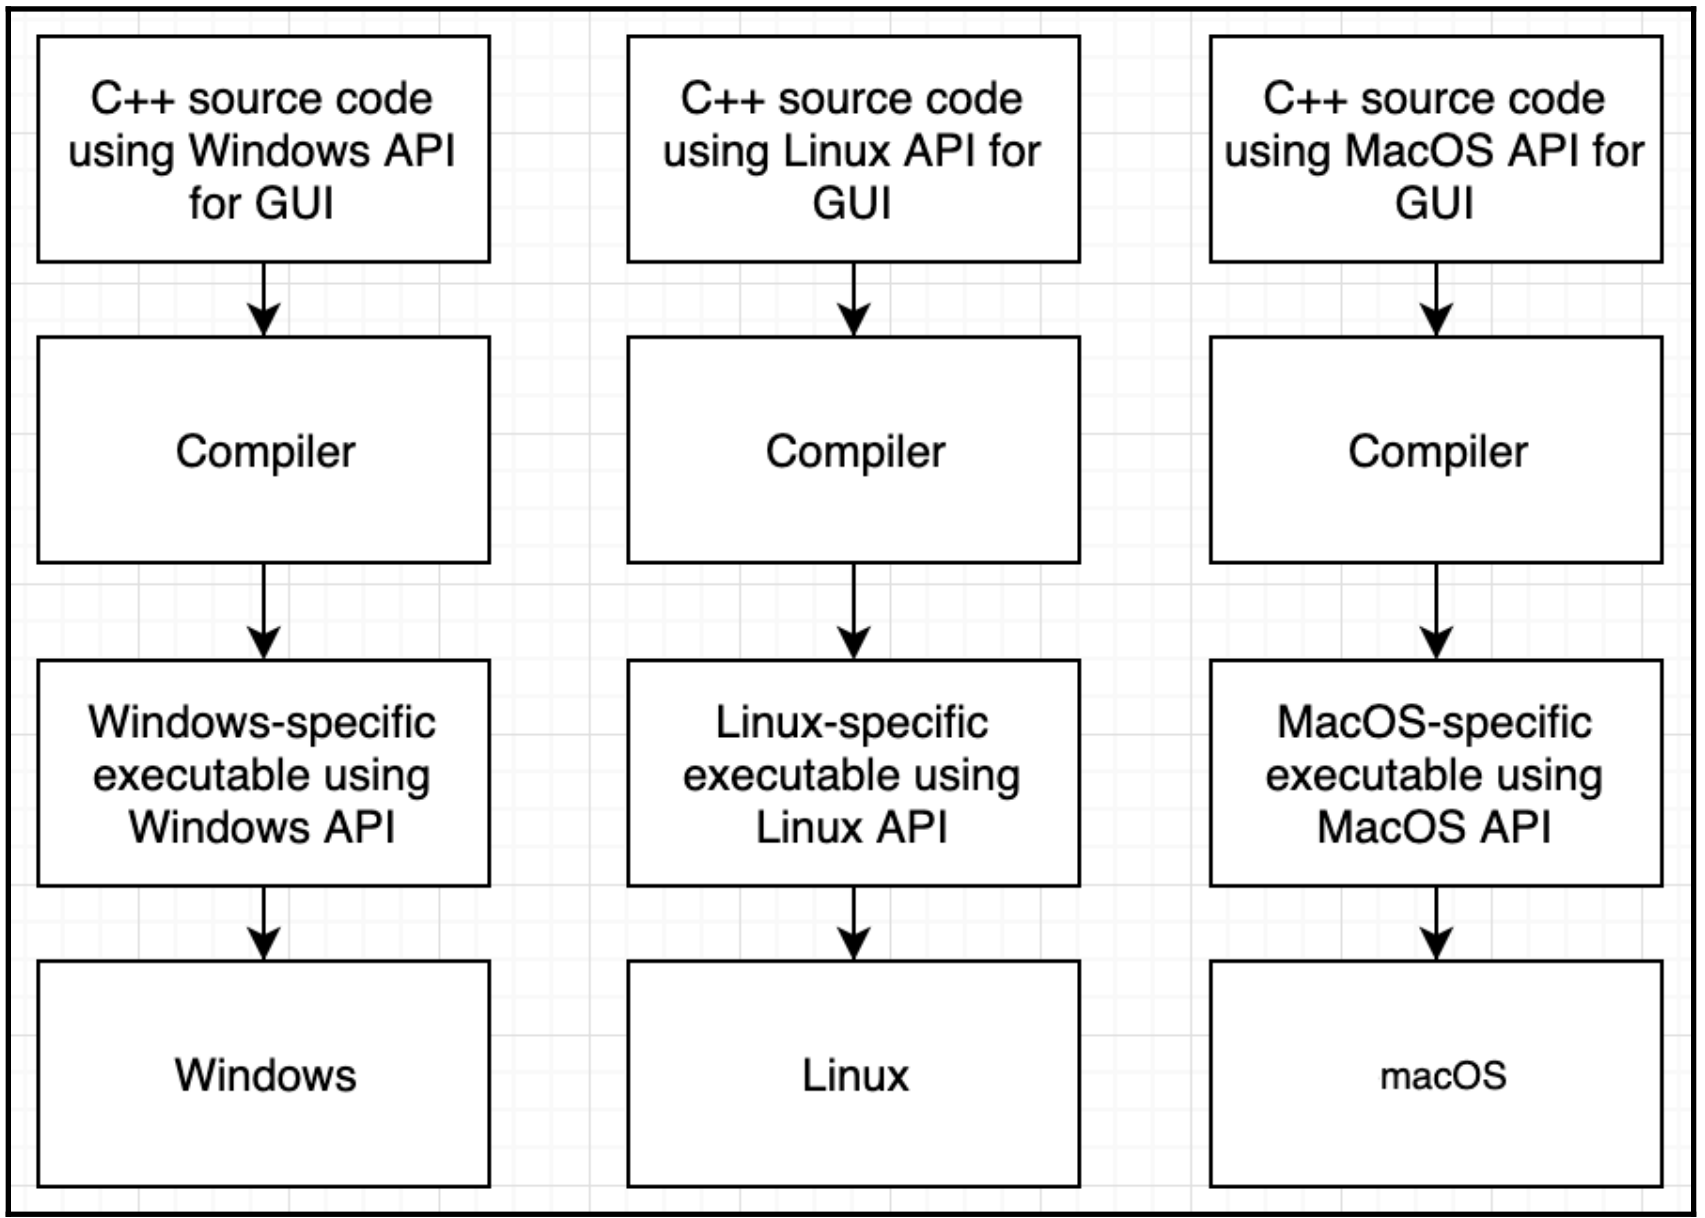
\includegraphics[width=1.0\textwidth]{content/Section-2/Chapter-14/3}
\end{center}

尽管应用程序逻辑、名称和任务可能是相同的,但它现在有三个不同的实现和三个不同的可执行文件。要将应用程序交付给最终用户,我们需要发现他们的操作系统并交付正确的可执行文件。在Web上下载应用程序时,可能遇到过类似的情况。他们提供基于操作系统的下载应用程序。这就是Qt要一展身手的地方,让我们一起来看看。 \par

\noindent\textbf{}\ \par
\textbf{Qt跨平台的模式} \ \par
Qt是一个流行的用于创建GUI应用程序的工具包。它允许我们创建运行在各种系统上的跨平台应用程序。Qt由以下模块组成: \par

\begin{itemize}
	\item Qt Core: 核心类
	\item Qt GUI: GUI组件的基类
	\item Qt Widgets: 用C++ widget扩展Qt GUI的类
	\item Qt Multimedia: 音频、视频、广播和相机功能的课程
	\item Qt Multimedia Widgets: 用于实现多媒体功能的类
	\item Qt Network: 网络编程类(我们将在本章中使用它们)
	\item Qt Modeling Language (QML): 用于构建具有自定义用户界面的应用程序的声明性框架
	\item Qt SQL: 使用SQL集成数据库的类
	\item Qt Quick family of modules: 本书中不会讨论的QML相关的模块。
	\item Qt Test: 用于单元测试Qt应用程序的类
\end{itemize}

程序中使用的每个模块都通过一个后缀为.pro的项目文件附加到编译器中。这个文件描述了qmake构建应用程序所需的所有内容,qmake是一个旨在简化构建过程的工具。描述项目的.pro文件中的项目组件(源代码、Qt模块、库等),例如:一个使用Qt Widgets和Qt网络的项目,由main.cpp和test.cpp文件组成,.pro文件的内容如下: \par

\begin{lstlisting}[caption={}]
QT += widgets
QT += network
SOURCES += test.cpp
SOURCES += main.cpp
\end{lstlisting}

我们也可以在. pro文件中指定特定于平台的源文件,如下所示: \par

\begin{lstlisting}[caption={}]
QT += widgets
QT += network
SOURCES += test.cpp
SOURCES += main.cpp
win32 {
	SOURCES += windows_specific.cpp
}
unix {
	SOURCES += linux_world.cpp
}
\end{lstlisting}

当我们在Windows环境中构建应用程序时,windows\underline{ }specific.cpp文件将参与构建。相反,在Unix环境中构建时,将包含linux\underline{ }world.cpp文件,忽略windows\underline{ }specific.cpp文件。至此,我们遇到了Qt应用程序的编译模型。 \par
Qt提供跨平台编程的强大能力的全部意义在于元编译源代码,在代码被传递给C++编译器之前,Qt编译器通过引入或替换特定于平台的组件来清理代码。例如,当我们使用一个按钮组件(QPushButton)时,如果在Windows环境中编译,它将被一个特定于Windows的按钮组件所取代。这就是为什么.pro文件也可以包含项目特定于平台的修改。下面的图表描述了这一过程: \par

\begin{center}
	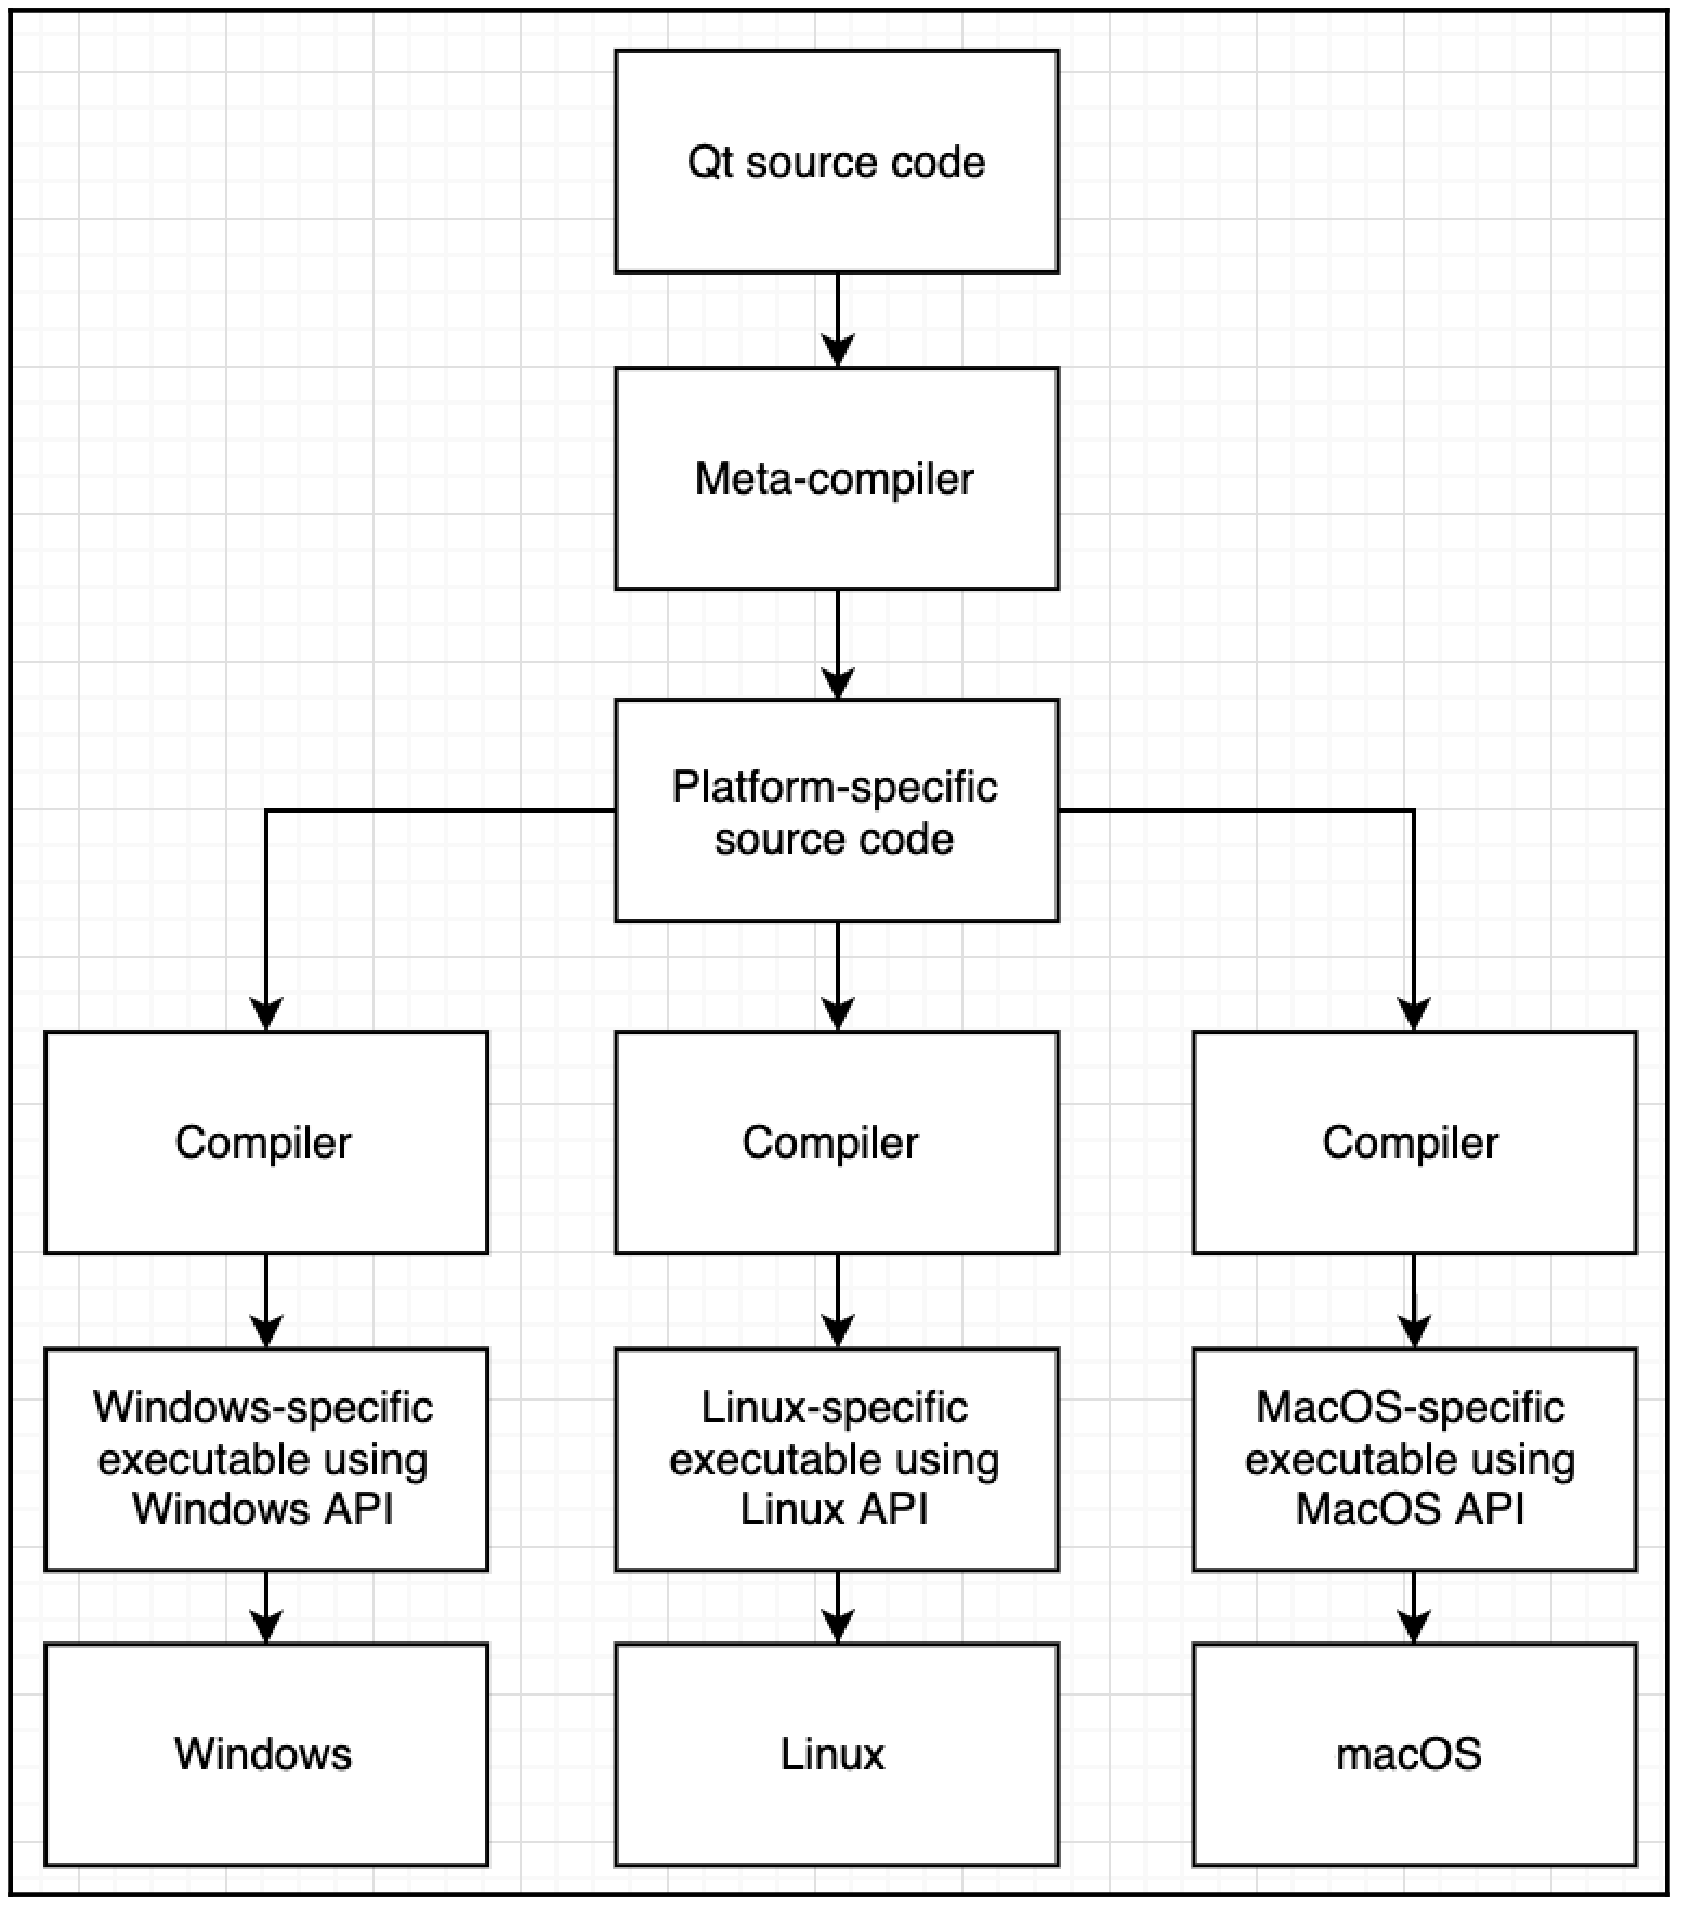
\includegraphics[width=1.0\textwidth]{content/Section-2/Chapter-14/4}
\end{center}

元编译器通常称为元对象编译器(MOC)。这种方法的美妙之处在于,生成的输出代表了在没有虚拟机的情况下运行的相同的机器代码,我们可以马上发布这个可执行文件。这种方法的缺点是,对于不同的平台,我们有不同的可执行文件。然而,我们只编写一个应用程序——不需要使用不同的语言,不需要钻研特定于操作系统的API,也不需要学习特定于操作系统的GUI组件类名。就像Qt说的,\textit{Write once, compile everywhere}。现在,让我们继续构建一个简单的GUI应用程序。 \par

\noindent\textbf{}\ \par
\textbf{编写一个简单的应用程序} \ \par
我们不会讨论提到的所有模块,因为这需要一本全新的书来进行。你可以参考本章末尾列出的书,在扩展阅读部分,以获得更多信息。主函数是这样的: \par

\begin{lstlisting}[caption={}]
#include <QtWidgets>

int main(int argc, char** argv)
{
	QApplication app(argc, argv);
	
	QPushButton btn("Click me!");
	btn.show();
	return app.exec();
}
\end{lstlisting}

让我们看看代码中使用的各种组件。第一个是QtWidgets头文件,它包含widget组件,我们可以使用这些组件为应用程序构建细粒度的GUI。接下来是QPushButton类,它表示可单击按钮的包装器。我们在这里有意地把它作为一个包装器来介绍,以便在本章后面讨论Qt程序的编译过程时能够解释它。下面是运行上述代码的结果: \par

\begin{center}
	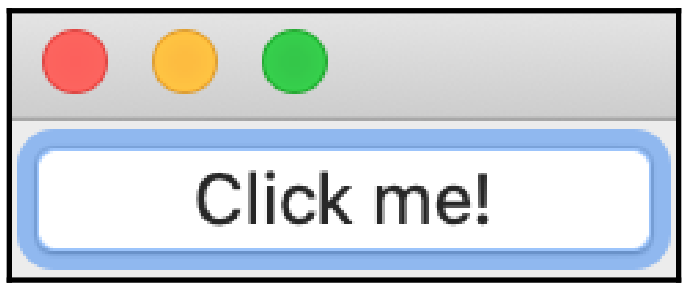
\includegraphics[width=0.4\textwidth]{content/Section-2/Chapter-14/5}
\end{center}

我们只声明了QPushButton类,但它显示为一个带有操作系统标准的关闭和最小化按钮的窗口(在示例中,这是macOS)。这样做的原因是QPushButton间接继承自QWidget,它是一个带有框架的widget,也就是一个窗口。这个按钮几乎占据了整个窗口的空间。我们可以调整窗口的大小,看看按钮是如何随它一起调整大小的。我们将在本章后面更详细地讨论widget。 \par
当我们运行app.exec()时,GUI就会构建。注意app对象的类型。它是一个QApplication对象。这是Qt应用程序的起点。当我们调用exec()函数时,我们开始Qt的事件循环。为了理解GUI应用程序的生命周期,我们应该稍微改变一下对程序执行的看法。在第7章之后,重新定义程序构造和执行的概念并不奇怪这里需要了解的主要内容是GUI应用程序有一个与主程序一起运行的额外实体。这个实体称为事件循环。 \par

\hspace*{\fill} \\ %插入空行

\includegraphics[width=0.05\textwidth]{images/tip}
回想一下我们在第11章中讨论过的事件循环。这个游戏代表了一个带有视觉组件的程序,用户可以与这些组件进行密集的交互。这同样适用于带有按钮、标签和其他图形组件的常规GUI应用程序。 \par
\noindent\textbf{}\ \par

用户与应用程序交互,用户的每个操作都解释为一个事件,然后将每个事件推入队列。事件循环一个接一个地处理这些事件。处理事件意味着调用附加在事件上的特殊处理函数,例如:每当单击一个按钮时,就会调用keyPressedEvent()函数。它是一个虚函数,所以我们可以在设计自定义按钮时覆盖它,代码如下所示: \par

\begin{lstlisting}[caption={}]
	class MyAwesomeButton : public QPushButton
	{
		Q_OBJECT
		public:
		void keyPressedEvent(QKeyEvent* e) override
		{
			// anything that we need to do when the button is pressed
		}
	};
\end{lstlisting}

事件的唯一参数是指向QKeyEvent的指针,QEvent的子类型。QEvent是Qt中所有事件类的基类,注意在类的开始块后面放置了一个奇怪的Q\underline{ }OBJECT。这是一个Qt特有的宏,如果想让Qt的MOC发现,应该把它放在自定义类的第一行。 \par
下一节中,我们将介绍Qt对象特有的信号和槽机制。为了使我们的自定义对象支持这种机制,我们在类定义中放置Q\underline{ }OBJECT宏。 \par
现在,让我们构建一个比简单按钮更大的东西。下面的例子创建了一个标题为Mastering C++的窗口: \par

\begin{lstlisting}[caption={}]
	#include <QtWidgets>
	int main(int argc, char** argv)
	{
		QApplication app(argc, argv);
		
		QWidget window;
		window.resize(120, 100);
		window.setWindowTitle("Mastering C++");
		window.show();
		
		return app.exec();
	}
\end{lstlisting}

下面是我们通过执行前面的程序得到的结果: \par

\begin{center}
	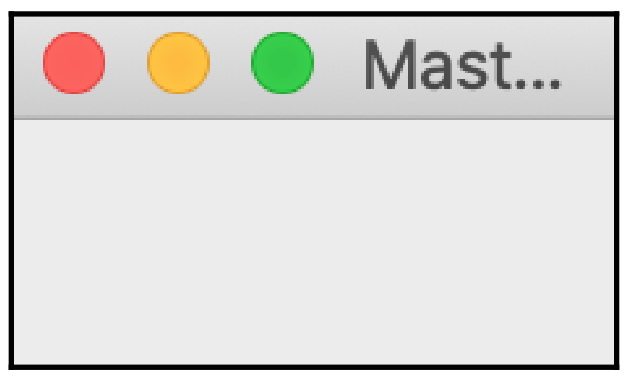
\includegraphics[width=0.3\textwidth]{content/Section-2/Chapter-14/6}
\end{center}

标题部分没有显示完全。现在,如果我们手动调整它的大小或更改源代码,使其在resize()函数的第二个参数中具有更大的值,我们会得到以下结果: \par

\begin{center}
	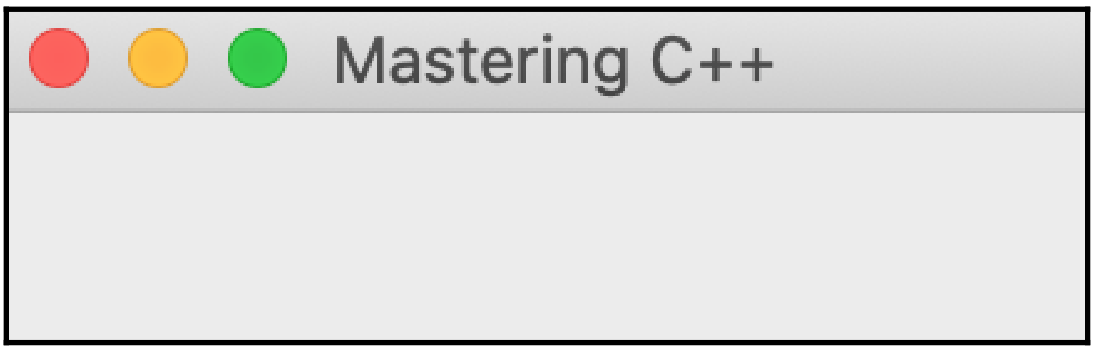
\includegraphics[width=0.4\textwidth]{content/Section-2/Chapter-14/7}
\end{center}

窗口对象是QWidget类型的。QWidget是所有用户界面对象的中心类。无论何时您想要创建一个自定义widget或扩展一个现有的widget,您都可以直接或间接地从QWidget继承。它为每个用例提供了很多功能。您可以使用move()函数在屏幕中移动它,也可以通过调用showFullScreen()使窗口全屏等。在前面的代码中,我们调用了resize()函数,该函数获取widget的宽度和高度以调整其大小。另外,请注意setWindowTitle()函数,它执行tin上所说的操作——它将传递的字符串参数设置为窗口的标题。在代码中使用字符串值时,最好使用QApplication::translate()函数。它使程序的本地化变得更容易,因为当语言设置改变时,Qt会自动用正确的翻译替换文本。QObject::tr()提供了相同的功能。 \par

\hspace*{\fill} \\ %插入空行

\includegraphics[width=0.05\textwidth]{images/warn}
QObject是所有Qt类型的基类。在Java或C\#这样的语言中,每个对象都直接或间接地继承自泛型类型,大多数是命名对象(C++不包含公共基类)。另一方面,Qt引入了QObject,它附带了所有对象都应该支持的基本功能。 \par
\noindent\textbf{}\ \par

现在我们已经接触了Qt应用程序开发的基础知识,让我们深入了解一下这个框架并发现它的关键特性。 \par

\noindent\textbf{}\ \par
\textbf{研究Qt} \ \par
Qt随着时间的推移不断发展,在撰写本书时,它的版本是5.14。它的第一个公开预发行版本是在1995年宣布的。20多年过去了,现在Qt拥有很多功能强大的功能,这些功能几乎适用于所有平台,包括Android和iOS等移动系统。除了少数例外,我们可以满怀信心地用C++和Qt为所有平台编写功能齐全的GUI应用程序。这是一个重大的游戏规则改变者,因为公司雇佣的是专注于一种技术的小型团队,而不是针对每个特定平台组建多个团队。 \par
如果您是Qt的新手,强烈建议您尽可能地熟悉它(参阅本章末尾的书籍参考)。除了GUI框架提供的常规组件外,Qt还引入了一些新的或在框架中巧妙实现的概念。其中一个概念是使用信号和插槽的对象之间的通信。 \par

\noindent\textbf{}\ \par
\textbf{抓取信号和槽} \ \par
Qt引入了信号和槽的概念,作为对象之间的通信机制。信号和槽的概念及其实现机制是Qt与其他GUI框架区别开来的特性之一。前面的章节中,我们讨论了观察者模式。该模式的主要思想是使用一个对象将事件通知给其他对象(订阅者)。信号和槽的机制类似于观测器模式的实现。它是一个对象通知另一个对象它的变化的一种方式。Qt提供了一个通用接口,可以通过将一个对象的信号绑定到另一个对象的插槽来将对象连接在一起。信号和槽都是对象的常规成员函数。信号是针对对象的指定操作调用的函数。槽位是作为订阅器的另一个功能。它由信号函数调用。 \par
正如我们前面提到的,Qt向我们介绍了所有对象的基类型QObject。支持信号和槽的基本功能在QObject中实现。在代码中声明的任何对象、QWidget、QPushButton等都继承自QObject,因此它们都支持信号和槽。QObject为我们提供了两个管理对象通信的函数,分别是connect()和disconnect(): \par

\begin{lstlisting}[caption={}]
bool connect(const QObject* sender, const char* signal,
	const QObject* receiver, const char* method,
	Qt::ConnectionType type = Qt::AutoConnect);

bool disconnect(const QObject* sender, const char* signal,
	const QObject* receiver, const char* method);
\end{lstlisting}

如您所见,connect()函数将接收方和发送方对象作为参数。此外,它还接受信号和槽的名称。信号是与发送方相关联的,而插槽是接收方提供的。下图说明了这一点:  \par

\begin{center}
	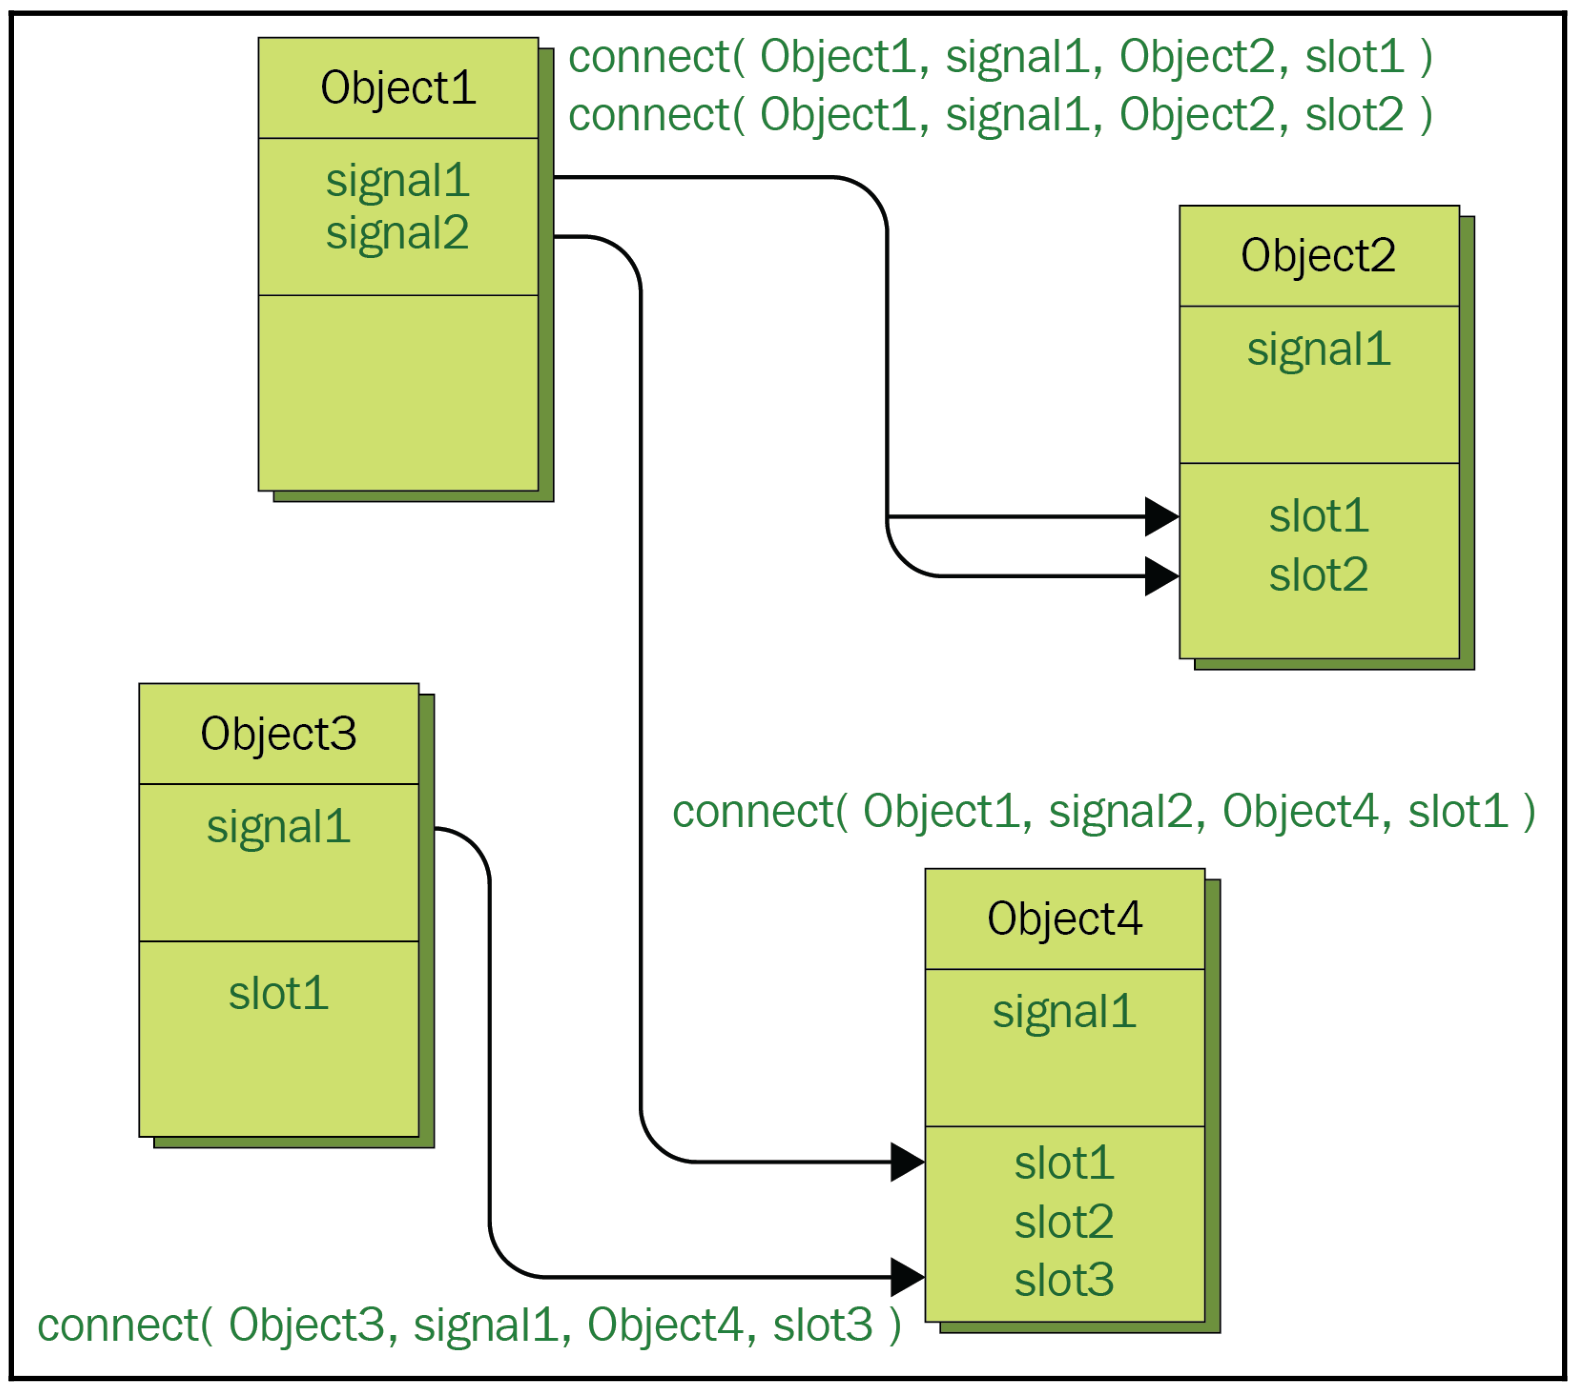
\includegraphics[width=1.0\textwidth]{content/Section-2/Chapter-14/8}
\end{center}

编写Qt应用程序时,使用信号和槽操作将变得很自然。另外,注意信号和槽在connect()和disconnect()函数中处理为字符串。要在连接对象时指定信号和槽,我们需要使用另外两个宏:signal()和slot()(从现在开始不会再引入更多的宏)。 \par
下面是我们如何将两个物体连接在一起。假设我们想要更改标签(QLabel的一个实例)的文本,以便在单击按钮时接收到一个信号。为此,我们将QPushButton的clicked()信号连接到QLabel槽位,如下所示: \par

\begin{lstlisting}[caption={}]
QPushButton btn("Click me!");
QLabel lbl;
lbl.setText("No signal received");
QObject::connect(&btn, SIGNAL(clicked()), &lbl, SLOT(setText(const
QString&)));
\end{lstlisting}

前面的代码可能看起来有点冗长,可以把它看作是一种方便的信号和槽机制的付出。然而,前面的例子不会给出我们需要的结果,它不会设置标签的文本来声明它收到了信号。我们应该以某种方式将该字符串传递给标签的槽,clicked()信号不会为我们做这些。实现这一点的方法之一是扩展QLabel,使其实现一个自定义槽,设置文本接收信号。我们可以这样做: \par

\begin{lstlisting}[caption={}]
class MyLabel : public QLabel
{
	Q_OBJECT
	public slots:
	void setCustomText() {
		this->setText("received a signal");
	}
};
\end{lstlisting}

为了声明一个槽,就像我们在前面的代码中所做的那样。信号的声明方式几乎相同:用Signals指定,唯一的区别是信号不能是私有的或受保护的。我们就这样声明它们: \par

\begin{lstlisting}[caption={}]
class Example
{
	Q_OBJECT:
public:
	// member functions
public slots:
	// public slots
private slots:
	// private slots
signals: // no public, private, or protected
	// signals without any definition, only the prototype
};
\end{lstlisting}

现在,我们只需要更新前面的代码来改变标签的信号(以及标签对象的类型): \par

\begin{lstlisting}[caption={}]
QPushButton btn("Click me!");
MyLabel lbl;
lbl.setText("No signal received");
QOBject::connect(&btn, SIGNAL(clicked()), &lbl, SLOT(setCustomText()));
\end{lstlisting}

当信号发出时,将调用槽。也可以从对象中声明和发射信号。与信号和插槽相关的一个重要细节是,它们独立于GUI事件循环。 \par
当信号发出时,连接的槽立即执行。我们可以通过传递Qt::ConnectionType作为connect()函数的第五个参数来指定连接类型。它由以下值组成: \par

\begin{itemize}
	\item AutoConnection
	\item DirectConnection
	\item QueuedConnection
	\item BlockingQueuedConnection
	\item UniqueConnection
\end{itemize}

在DirectConnection中,信号发出时立即调用槽。另一方面,当使用QueuedConnection时,当执行返回到接收方对象的线程的事件循环时,将调用槽。BlockingQueuedConnection与QueuedConnection类似,不同之处在于会让线程被阻塞,直到槽返回一个值。自动连接可以是DirectConnection或QueuedConnection。如果接收端和发送端在同一个线程中,使用DirectConnection,否则,连接将使用QueuedConnection。最后,UniqueConnection与前面描述的任何连接类型一起使用(它使用位或与其中的一个组合),唯一目的是让connect()函数在信号和线程之间已经建立了连接时失败。 \par
信号和槽形成了一种强大的机制,使Qt成为GUI编程中出色的框架。我们要介绍的下一个机制在框架中很流行,它与我们在应用程序中操作数据的方式有关。 \par

\noindent\textbf{}\ \par
\textbf{了解编程模型/视图} \ \par
模型/视图编程起源于模型-视图-控制器(MVC)设计模式。该模式背后的主要思想是将问题分解为三个松散耦合的组件,如下所示: \par

\begin{itemize}
	\item 模型,负责存储和操作数据
	\item 视图,负责呈现和可视化数据
	\item 控制器,负责额外的业务逻辑,并提供从模型到视图的数据
\end{itemize}

通过它的发展,我们现在有了一种简化和更方便的编程方法,称为模型/视图编程。它与MVC模式相似,只是它省略了控制器,使视图和模型更关心手边的功能。我们可以说视图和控制器在模型/视图架构中结合在一起。看看下面的架构图: \par

\begin{center}
	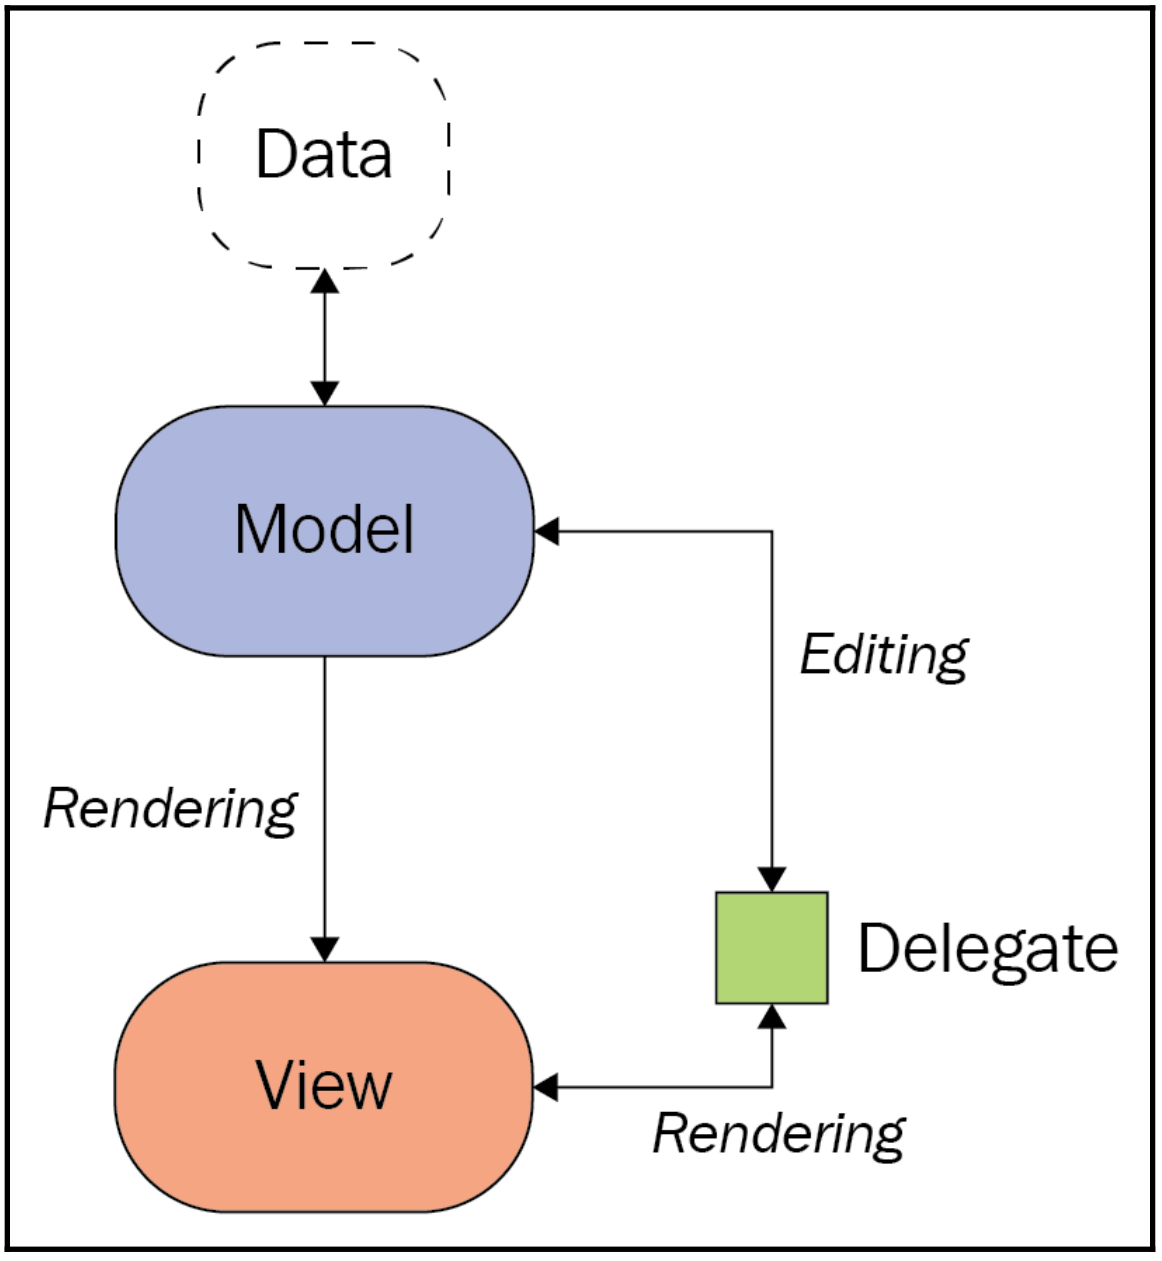
\includegraphics[width=0.8\textwidth]{content/Section-2/Chapter-14/9}
\end{center}

模型表示数据,数据与其源通信,并为体系结构中的其他组件提供了一个方便的接口。模型的实现及其与其他组件的通信基于数据类型。 \par
视图通过获得所谓的模型索引来获得对数据项的引用。视图可以检索并向模型提供数据。关键是,可以使用视图编辑数据项,委托扮演与模型通信以保持数据同步的角色。 \par
引入的每个组件——模型、视图和委托——都是由提供公共接口的抽象类定义。某些情况下,类还提供特性的默认实现。为了编写专门化的组件,我们从抽象类派生子类。当然,模型、视图和委托使用信号和槽进行通信,我们在前一节中介绍了这一点。 \par
当模型遇到数据中的更改时,它会通知视图。另一方面,用户与呈现数据项的交互是由视图发出的信号通知的。最后,来自委托的信号将数据编辑的状态通知模型和视图。 \par
模型基于QAbstractItemModel类,该类定义了视图和委托使用的接口。Qt提供了一组不需要修改就可以使用的现有模型类,但如果您需要创建新的模型,应该从QAbstractItemModel继承您的类。例如,QStringListModel、QStandardItemModel和QFileSystemModel类可以处理数据项。QStringListModel用于存储字符串项列表(表示为QString对象)。此外,还有一些方便使用SQL数据库的模型类。QSqlQueryModel、QSqlTableModel和QSqlRelationalTableModel允许我们在模型/视图约定的上下文中访问关系数据库。 \par
视图和代理也有相应的抽象类,即QAbstractItemView和QAbstractItemDelegate。Qt提供了可以立即使用的现有视图,如QListView、QTableView和QTreeView。这些是大多数应用程序处理的基本视图类型。QListView显示项目列表,QTableView显示表中的数据,QTreeView显示层次化列表中的数据。如果你想使用这些视图类,Qt建议从QAbstractListModel或QAbstractTableModel继承自定义模型,而不是子类化QAbstractItemModel。 \par
QListView、QTreeView和QTableView认为是核心类和低级类。还有一些更方便的类可以为新手Qt使用者提供更好的可用性——QListWidget、QTreeWidget和QTableWidget。我们将在本章的下一节看到使用widget的例子。在此之前,让我们看一个简单的QListWidget的运行示例: \par

\begin{lstlisting}[caption={}]
#include <QListWidget>

int main(int argc, char** argv)
{
	QApplication app(argc, argv);
	QListWidget* listWgt{new QListWidget};
	return app.exec();
}
\end{lstlisting}

将项目添加到列表widget的方法之一是创建它们,我们可以通过将列表widget设置为其所有者来实现。下面的代码中,我们声明了三个QListWidgetItem对象,每个对象都有一个名称,并与前面声明的列表widget相关联: \par

\begin{lstlisting}[caption={}]
new QListWidgetItem("Amat", listWgt);
new QListWidgetItem("Samvel", listWgt);
new QListWidgetItem("Leia", listWgt);
\end{lstlisting}

或者,我们可以声明一个item,然后将它插入到listwidget中: \par

\begin{lstlisting}[caption={}]
QListWidgetItem* newName{new QListWidgetItem};
newName->setText("Sveta");
listWgt->insertItem(0, newName);
\end{lstlisting}

insertItem()成员函数的第一个参数是要插入项目的行数。我们将Sveta项目放在列表的第一个位置。 \par
既然我们已经接触了行的概念,我们应该回到模型及其索引。模型将数据封装为数据项的集合。模型中的每个项都有一个由QModelIndex类指定的惟一索引。这意味着模型中的每个项都可以通过关联的模型索引访问。为了获得模型索引,我们需要使用index()函数。下图描述了一个以表状结构组织数据的模型: \par

\begin{center}
	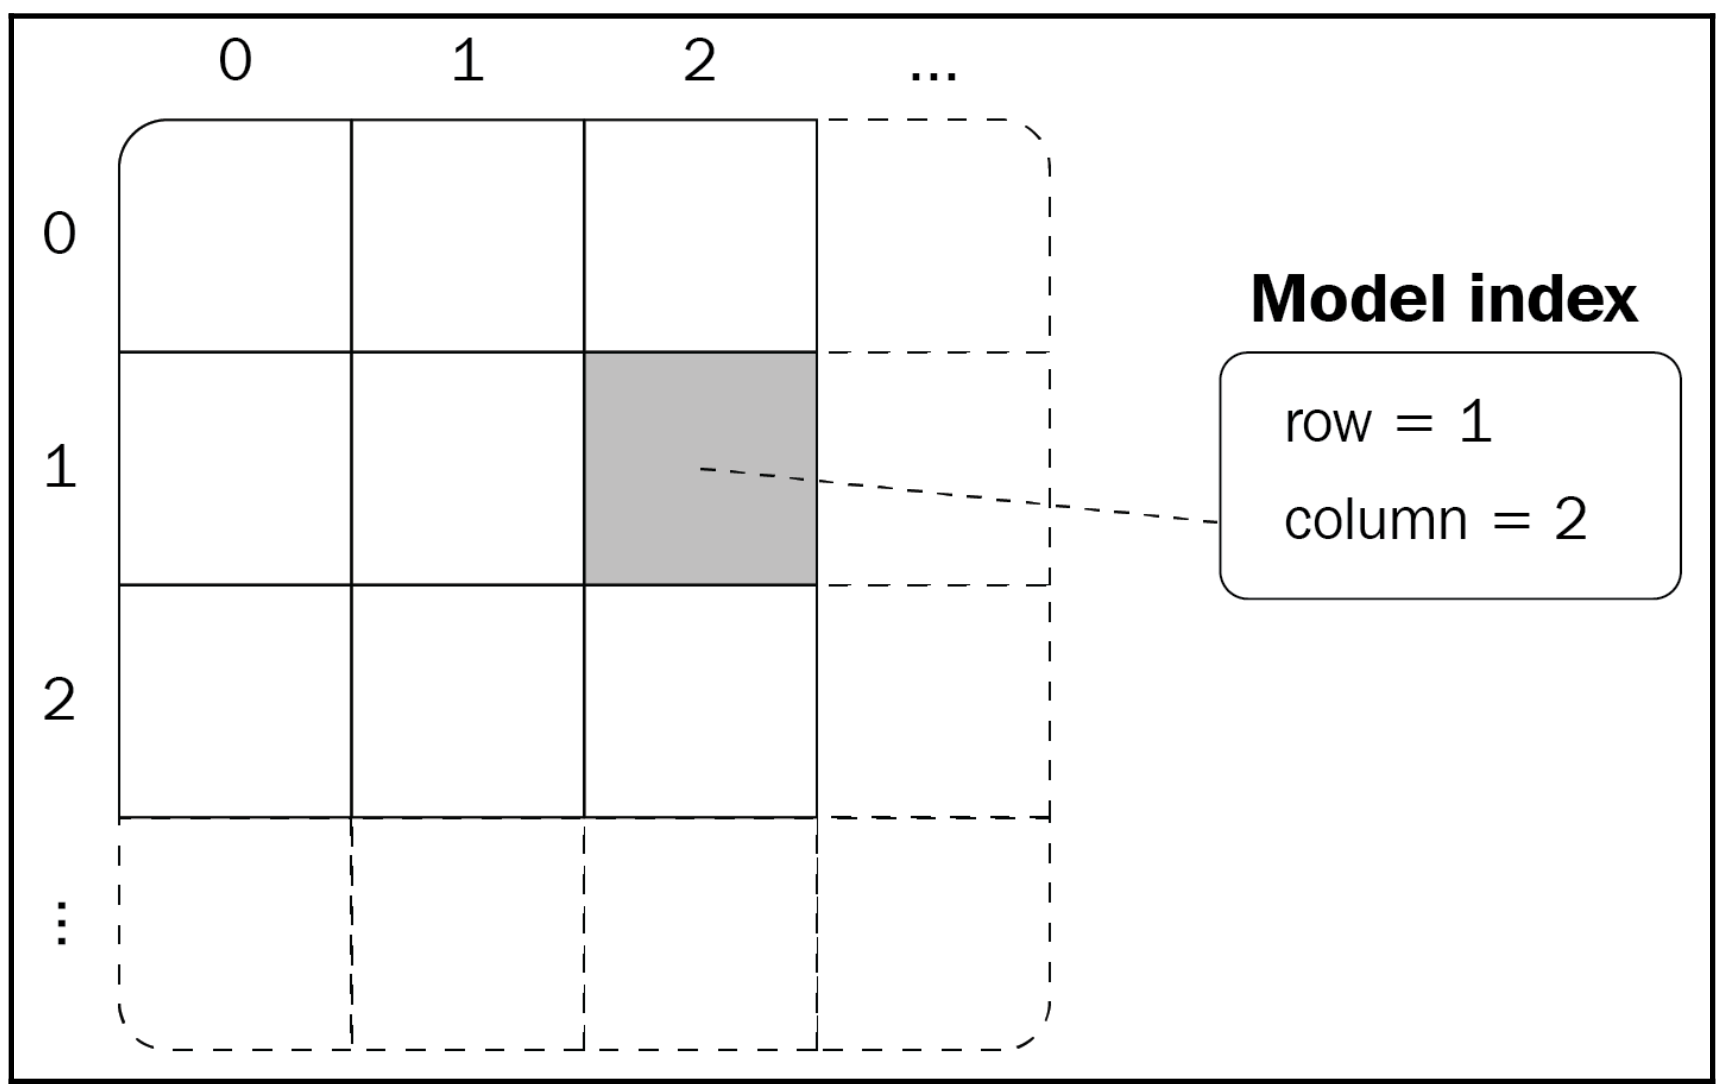
\includegraphics[width=1.0\textwidth]{content/Section-2/Chapter-14/10}
\end{center}

视图使用这种约定来访问模型中的数据项。但请注意,视图不受如何向用户显示数据的限制。由视图实现以方便用户的方式呈现和呈现数据。下图显示了数据在模型中的组织方式: \par

\begin{center}
	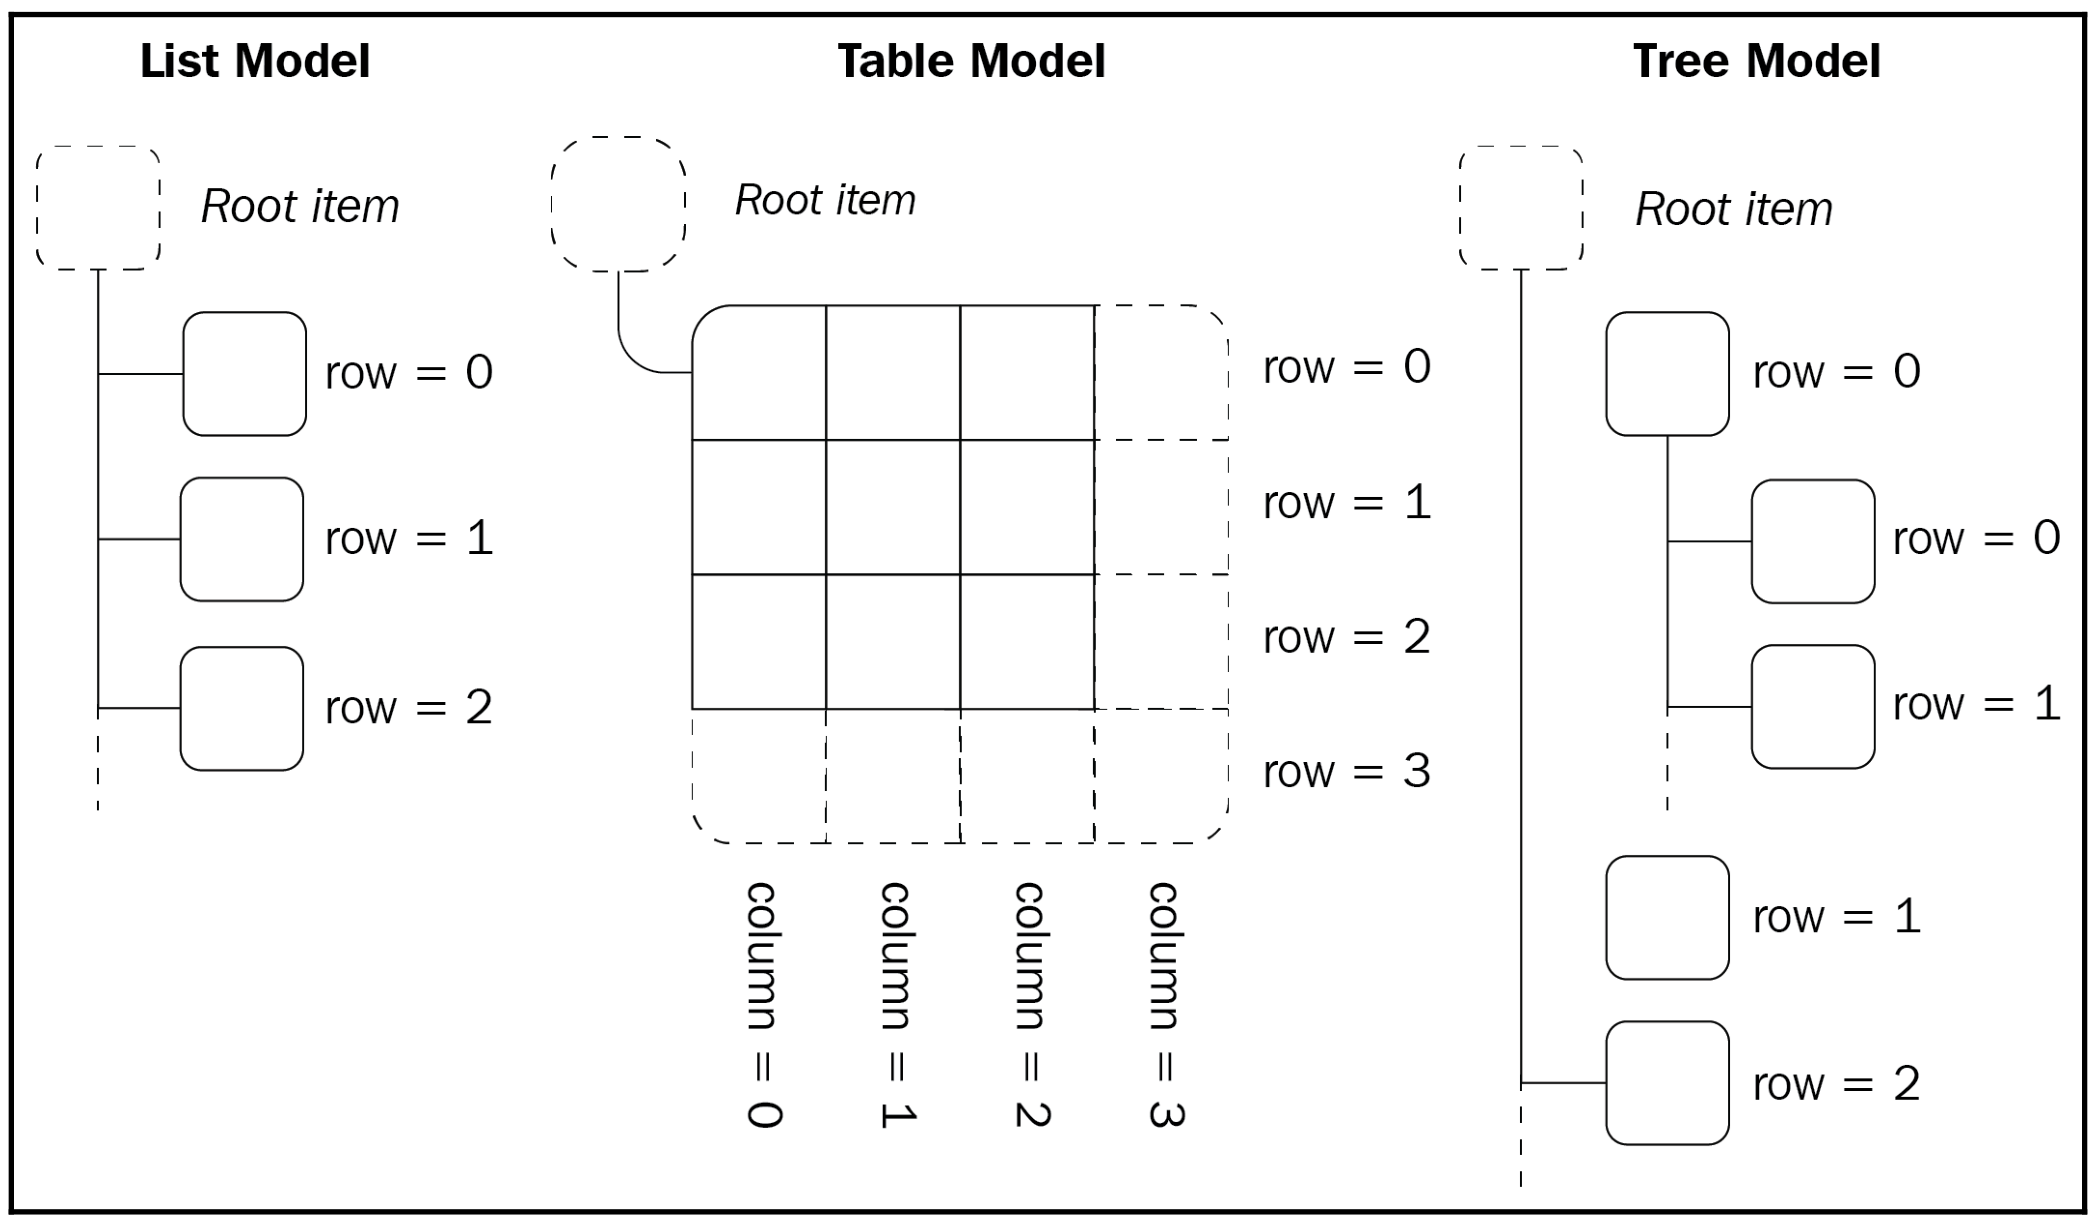
\includegraphics[width=1.0\textwidth]{content/Section-2/Chapter-14/11}
\end{center}

下面是我们如何使用模型索引访问第1行第2列的特定数据项: \par

\begin{lstlisting}[caption={}]
QModelIndex itemAtRow1Col2 = model->index(1, 2);
\end{lstlisting}

最后,让我们声明一个视图,并为它设置一个模型,以查看模型/视图编程的实际操作: \par

\begin{lstlisting}[caption={}]
QStringList lst;
lst << "item 1" << "item 2" << "item 3";

QStringListModel model;
model.setStringList(lst);

QListView lview;
lview.setModel(model);
\end{lstlisting}

在熟悉Qt提供的各种widget之后,我们将在下一节继续这个示例。 \par

\noindent\textbf{}\ \par
\textbf{使用Qtwidget} \ \par
widget是可视的GUI组件。如果一个widget没有父部件,它将被视为一个窗口,或者称为顶级widget。在本章的前面,我们在Qt中创建了一个尽可能简单的窗口,如下所示代码: \par

\begin{lstlisting}[caption={}]
#include <QtWidgets>

int main(int argc, char** argv)
{
	QApplication app(argc, argv);
	
	QWidget window;
	window.resize(120, 100);
	window.setWindowTitle("Mastering C++");
	window.show();
	
	return app.exec();
}
\end{lstlisting}

window对象没有父对象。问题是,QWidget的构造函数将另一个QWidget作为当前QWidget的父QWidget。因此,当我们声明一个按钮并希望它成为window对象的子对象时,我们可以这样做: \par

\begin{lstlisting}[caption={}]
#include <QtWidgets>

int main(int argc, char** argv)
{
	QApplication app(argc, argv);
	
	QWidget window;
	window.resize(120, 100);
	window.setWindowTitle("Mastering C++");
	window.show();
	
	QPushButton* btn = new QPushButton("Click me!", &window);
	return app.exec();
}
\end{lstlisting}

观察QPushButton构造函数的第二个参数。我们传递了一个窗口对象的引用作为它的父对象。当父对象被销毁时,它的子对象会自动销毁。Qt还支持许多其他widget,让我们来看看其中的一些。 \par

\noindent\textbf{}\ \par
\textbf{常见的Qtwidget} \ \par
上一节中,我们介绍了QPushButton类,并说明了它间接继承了QWidget类。为了创建一个窗口,我们使用QWidget类。结果是,QWidget代表了呈现到屏幕的能力,它是所有widget继承的基本类。它有很多属性和函数,比如enabled,一个boolean属性,如果widget启用,该属性为true。要访问它,我们使用isEnabled()和setEnabled()函数。为了控制widget的大小,我们使用它的高度和宽度,这表示widget的高度和宽度。为了获得它们的值,我们分别调用height()和width()。要设置新的高度和宽度,应该使用resize()函数,该函数接受两个参数——宽度和高度。还可以使用setMinimumWidth()、setMinimumHeight()、setMaximumWidth()和setMaximumHeight()函数来控制widget的最小和最大尺寸。当在布局中设置widget时,这可能会很有用(请参阅下一节)。除了属性和函数外,我们主要对QWidget的公共槽感兴趣,具体如下: \par

\begin{itemize}
	\item close() :关闭widget。
	\item hide() : 与setVisible(false)相同,这个函数隐藏了widget。
	\item lower()和raise() :在父部件的堆栈中移动widget(到底部或顶部)。每个widget都可以有一个父部件。没有父窗口widget的widget将成为一个独立窗口。我们可以使用setWindowTitle()和setWindowIcon()函数为这个窗口设置一个标题和一个图标。
	\item style:该属性保存widget的样式。为了修改它,我们使用setStyleSheet()函数传递描述widget样式的字符串。另一种方法是调用setStyle()函数并传递封装与样式相关属性的QStyle类型对象。
\end{itemize}

Qt部件几乎拥有所有必要的属性,可以开箱即用。很少会遇到必须构建自己的widget的情况。然而,有些团队为他们的软件创建了一整套定制widget。如果您计划为程序定制外观,那么这是很好的。例如,可以合并平面样式的widget,这意味着您必须修改框架提供的默认widget的样式。自定义widget应该继承自QWidget(或其任何后代),如下所示: \par

\begin{lstlisting}[caption={}]
class MyWidget : public QWidget
{};
\end{lstlisting}

如果希望widget公开信号和槽,则需要在类声明的开头使用Q\underline{ }OBJECT宏。更新后的MyWidget类的定义如下: \par

\begin{lstlisting}[caption={}]
class MyWidget : public QWidget
{
Q_OBJECT
public:
	// public section
signals:
	// list of signals
public slots:
	// list of public slots
};
\end{lstlisting}

正如您可能已经猜到的,信号没有访问修饰符,而槽可以分为公共、私有和受保护的部分。正如我们前面提到的,Qt提供了足够的开箱即用的widget。为了研究widget集,Qt提供了一组将widget组合在一起的示例。如果您已经安装了Qt Creator(用于开发Qt应用程序的IDE),那么您应该能够在一次单击中浏览这些示例。下面是它在Qt Creator中看起来的样子: \par

\begin{center}
	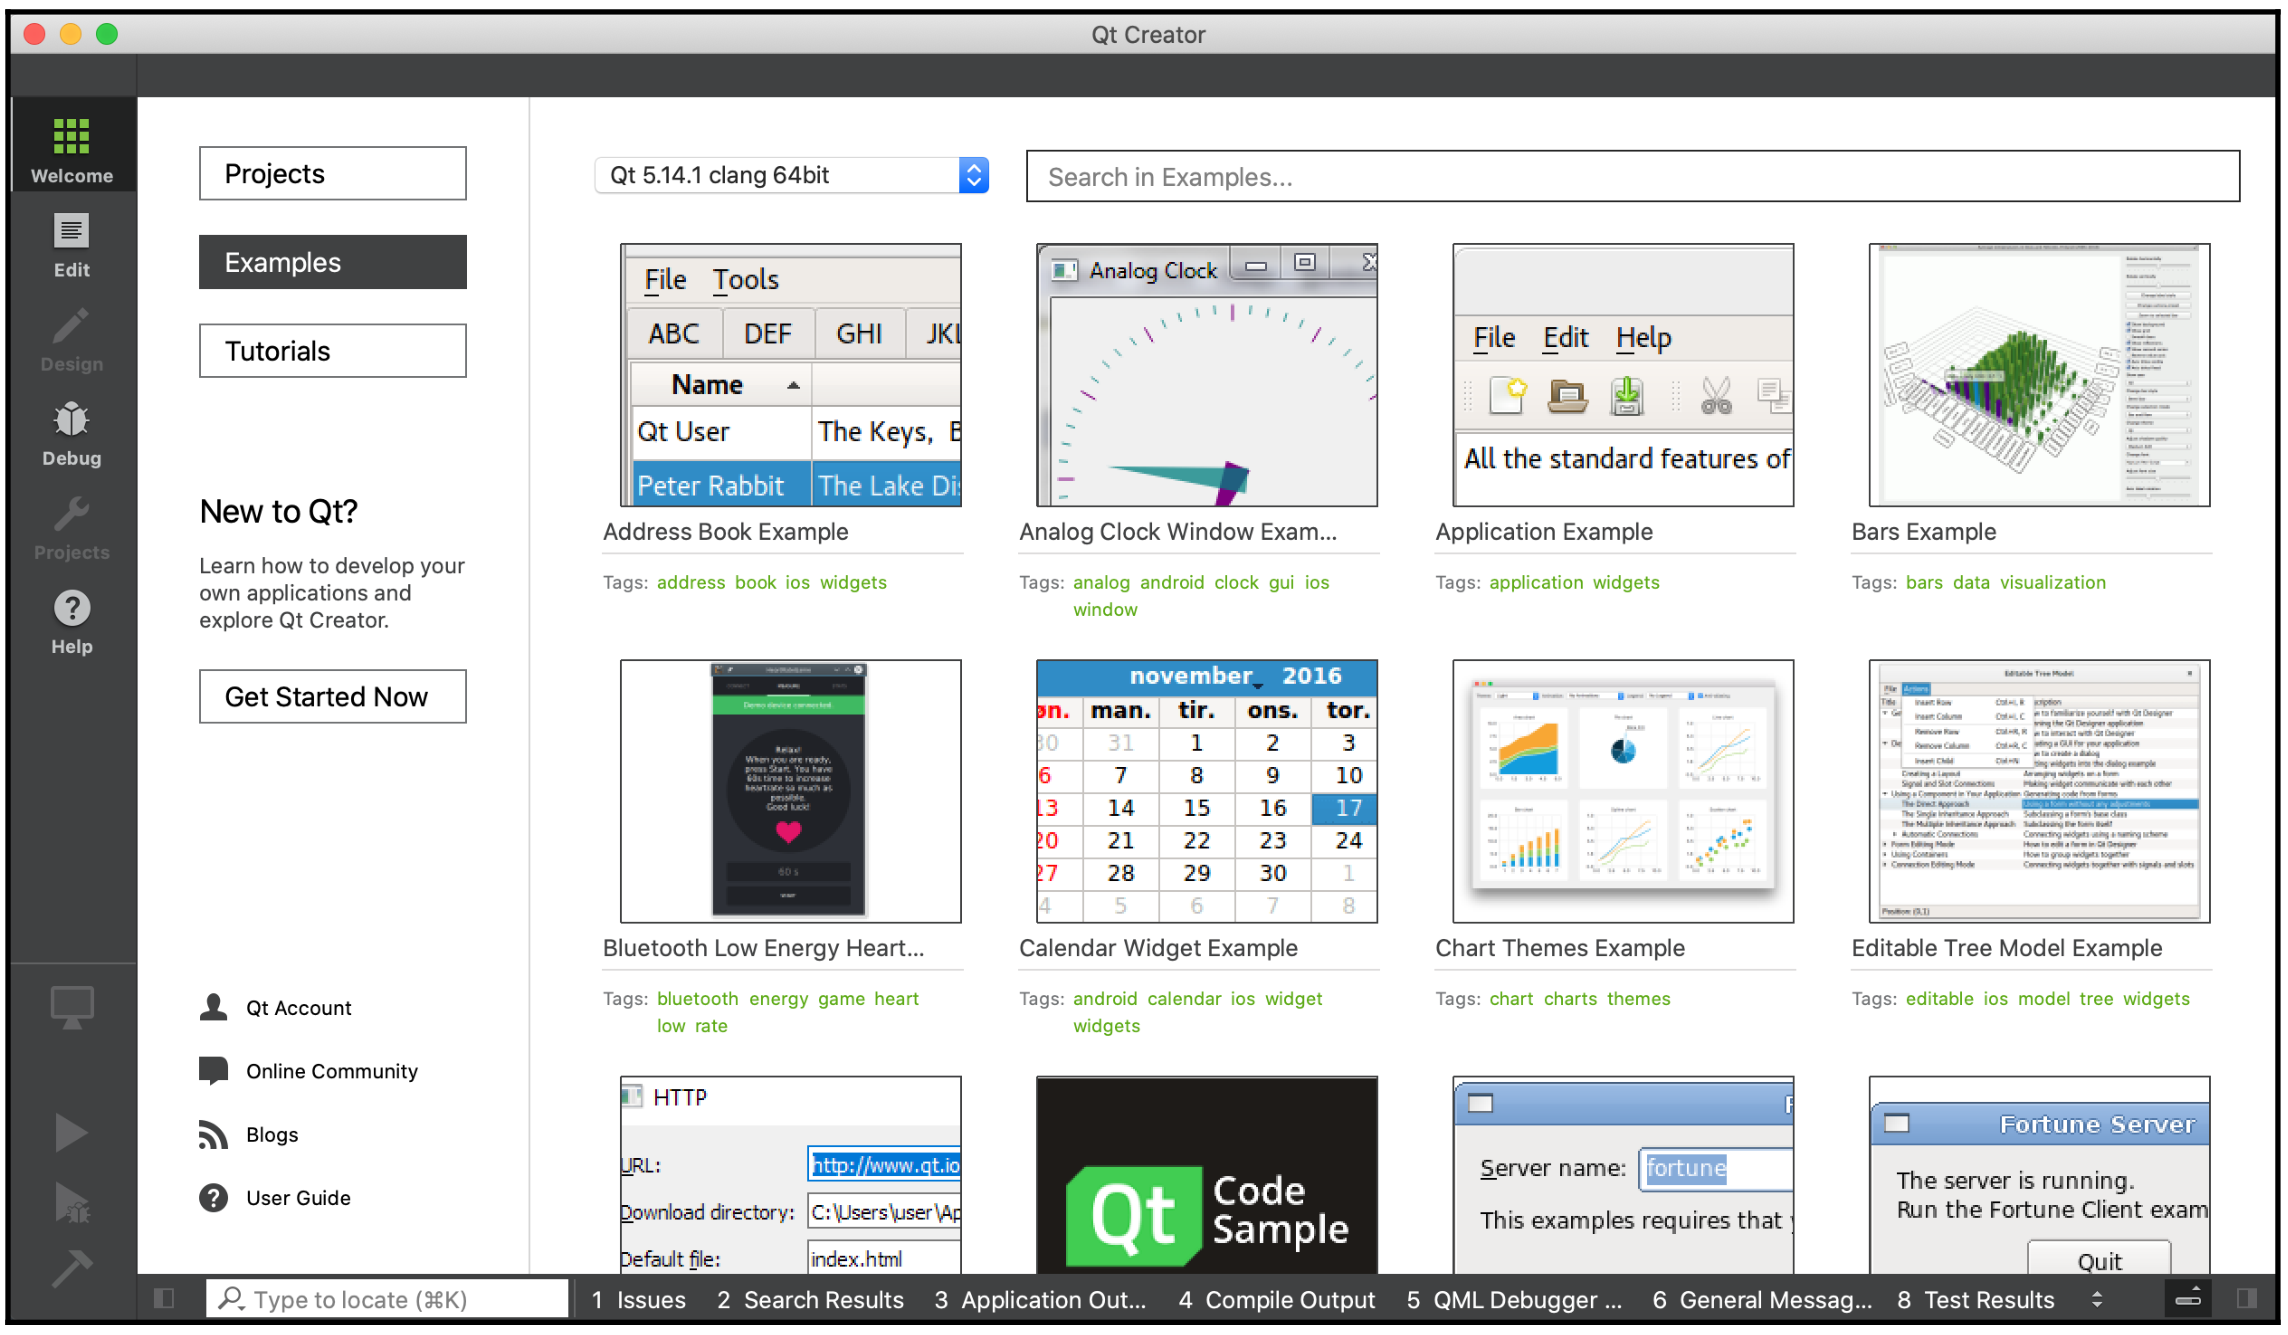
\includegraphics[width=1.0\textwidth]{content/Section-2/Chapter-14/12}
\end{center}

配置和运行地址簿的例子将给我们如下的接口: \par

\begin{center}
	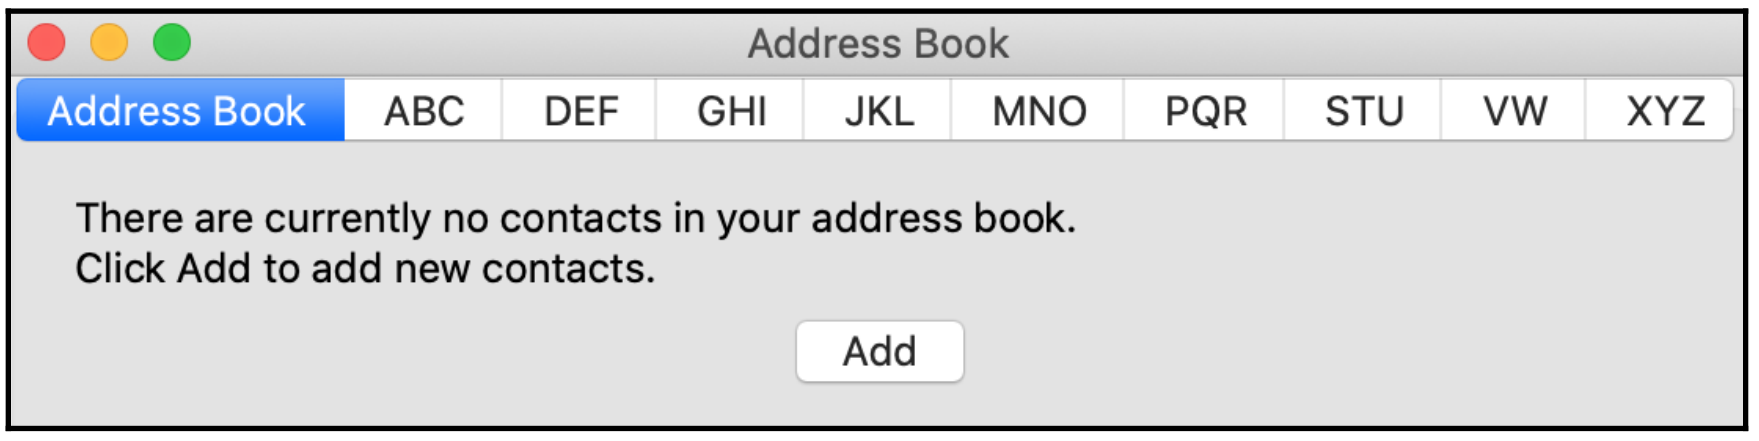
\includegraphics[width=0.8\textwidth]{content/Section-2/Chapter-14/13}
\end{center}

点击Add按钮将打开一个对话框,我们可以添加一个新的条目到地址簿,如下所示: \par

\begin{center}
	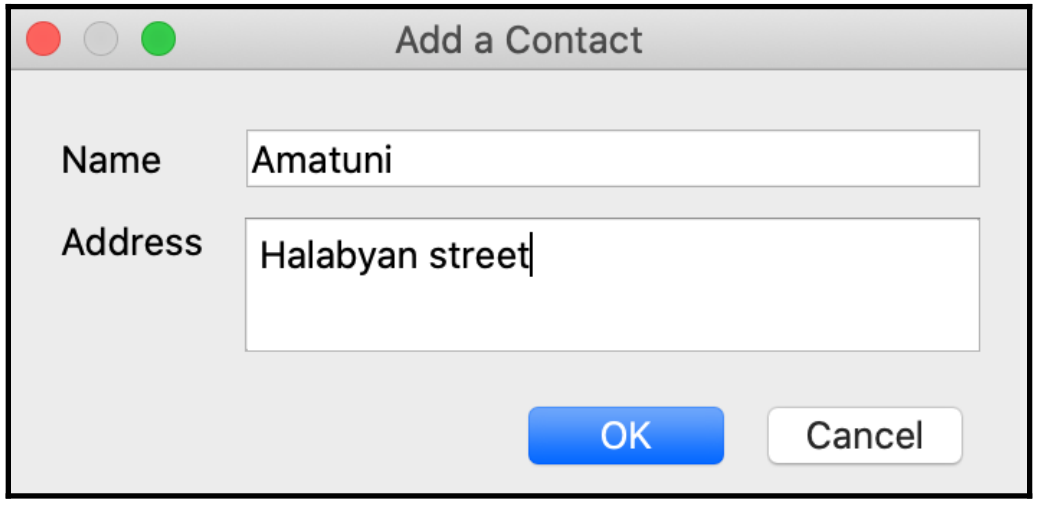
\includegraphics[width=0.8\textwidth]{content/Section-2/Chapter-14/14}
\end{center}

在添加了一些条目后,主窗口以表格的形式显示条目,如下所示: \par

\begin{center}
	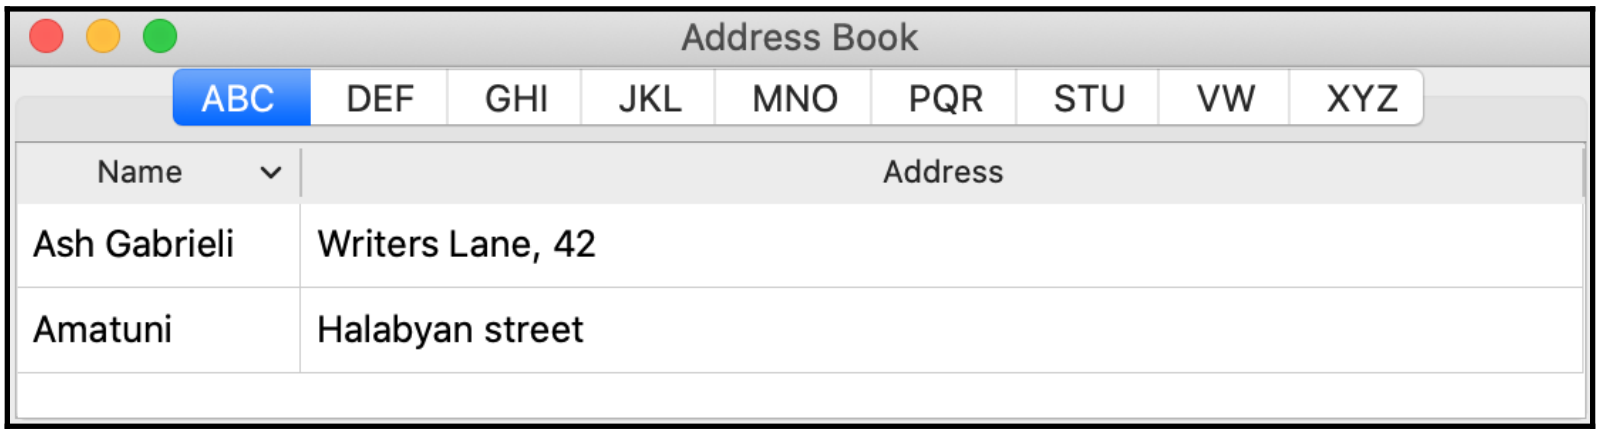
\includegraphics[width=0.8\textwidth]{content/Section-2/Chapter-14/15}
\end{center}

前面的屏幕截图显示了在一个应用程序中组合在一起的各种widget。以下是我们在GUI应用程序开发中经常使用的一些最常见的widget: \par

\begin{itemize}
	\item QCheckBox : 表示带有文本标签的复选框。
	\item QDateEdit : 表示可用于输入日期的widget。如果想要输入时间,也可以使用QDateTimeEdit。
	\item QLabel : 文本显示。也用于显示图像。
	\item QLineEdit :一个单行编辑框。
	\item QProgressBar : 呈现一个垂直或水平的进度条。
	\item QTabWidget : 作为标签widget的堆栈。这是许多组织者widget中的一个。其他一些是QButtonGroup、QGroupBox和QStackedWidget。
\end{itemize}

前面的列表不是最终的,但是它给出了Qt功能的基本概念。我们这里使用的地址簿示例使用了许多这样的widget。QTabWidget表示一个组织widget,将几个widget分组在一起。另一种组织widget的方法是使用布局。在下一节中,我们将介绍如何将widget组织在一起。 \par

\noindent\textbf{}\ \par
\textbf{使用布局组合widget} \ \par
Qt为我们提供了一个灵活而简单的平台,我们可以在这个平台上以布局的形式使用widget排布。这有助于我们确保widget内部的空间得到有效利用,并提供友好的用户体验。 \par
让我们来看看布局管理类的基本用法。使用布局管理类的优点是,当容器widget改变其大小时,它们会自动调整widget的大小和位置。Qt的布局类的另一个优点是,它们允许我们通过编写代码而不是使用UI编写器来安排widget。虽然Qt Creator提供了一种很好的手工组合widget(在屏幕上拖放widget)的方法,但大多数程序员在实际编写代码来安排widget的外观和感觉时,会感觉更舒服。假设你也喜欢后一种方法,我们将引入以下布局类: \par

\begin{itemize}
	\item QHBoxLayout
	\item QVBoxLayout
	\item QGridLayout
	\item QFormLayout
\end{itemize}

所有这些类都继承自QLayout,它是几何管理的基类。QLayout是继承自QObject的抽象基类。它没有继承自QWidget,因为它与渲染没有任何关系,但它负责组织应该呈现在屏幕上的widget。你可能不需要实现你自己的布局管理器,但如果做了,应该继承你的类从QLayout和提供实现以下函数: \par

\begin{itemize}
	\item addItem()
	\item sizeHint()
	\item setGeometry()
	\item itemAt()
	\item takeAt()
	\item minimumSize()
\end{itemize}

这里列出的类足以组成几乎任何复杂性的widget。更重要的是,我们可以将一种布局放置到另一种布局中,从而实现更灵活的widget组合。使用QHBoxLayout,我们可以从左到右水平地组织widget,如下图所示: \par

\begin{center}
	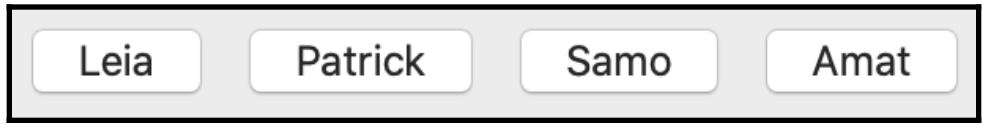
\includegraphics[width=0.6\textwidth]{content/Section-2/Chapter-14/16}
\end{center}

为了实现上述组合,我们需要使用以下代码: \par

\begin{lstlisting}[caption={}]
QWidget *window = new QWidget;
QPushButton *btn1 = new QPushButton("Leia");
QPushButton *btn2 = new QPushButton("Patrick");
QPushButton *btn3 = new QPushButton("Samo");
QPushButton *btn4 = new QPushButton("Amat");

QHBoxLayout *layout = new QHBoxLayout;
layout->addWidget(btn1);
layout->addWidget(btn2);
layout->addWidget(btn3);
layout->addWidget(btn4);

window->setLayout(layout);
window->show();
\end{lstlisting}

看一下我们在widget上调用setLayout()函数的那一行。每个widget都可以分配一个布局。如果没有容器,布局本身就不能发挥多大作用,因此我们需要将其设置为一个widget,作为有组织的widget(在本例中是按钮)的容器。QHBoxLayout继承自QBoxLayout,它有我们前面列出的另一个后代——QVBoxLayout。它类似于QHBoxLayout,但垂直组织部件,如下图所示: \par

\begin{center}
	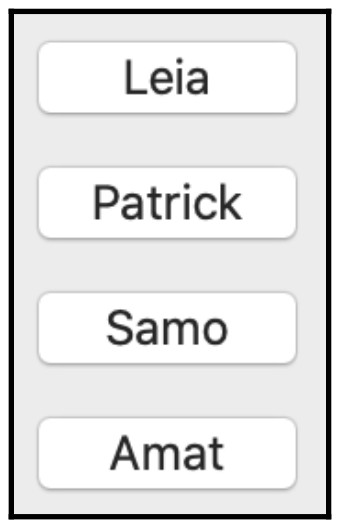
\includegraphics[width=0.4\textwidth]{content/Section-2/Chapter-14/17}
\end{center}

前面的代码中,我们唯一需要做的是用QVBoxLayout替换QHBoxLayout,如下所示: \par

\begin{lstlisting}[caption={}]
QVBoxLayout* layout = new QVBoxLayout;
\end{lstlisting}

GridLayout允许我们将widget组织成网格,如下图所示: \par

\begin{center}
	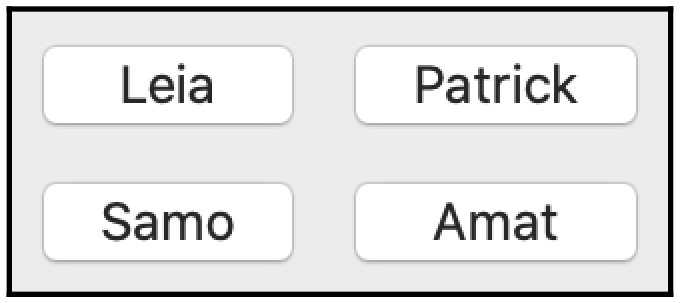
\includegraphics[width=0.6\textwidth]{content/Section-2/Chapter-14/18}
\end{center}

这是相应的代码: \par

\begin{lstlisting}[caption={}]
QGridLayout *layout = new QGridLayout;
layout->addWidget(btn1, 0, 0);
layout->addWidget(btn2, 0, 1);
layout->addWidget(btn3, 1, 0);
layout->addWidget(btn4, 1, 1);
\end{lstlisting}

最后,与QGridLayout类似,QFormLayout在设计输入表单时更有帮助,因为它以两列描述性样式布局widget。 \par
我们可以将一个布局组合到另一个布局中。为此,我们需要使用addItem()函数,如下所示: \par

\begin{lstlisting}[caption={}]
QVBoxLayout *vertical = new QVBoxLayout;
vertical->addWidget(btn1);
vertical->addWidget(btn2);

QHBoxLayout *horizontal = new QHBoxLayout;
horizontal->addWidget(btn3);
horizontal->addWidget(btn4);

vertical->addItem(horizontal);
\end{lstlisting}

布局管理器足够灵活,并且可以构建复杂的用户界面。 \par

\noindent\textbf{}\ \par
\textbf{总结} \ \par
如果你是Qt的新手,这一章可以作为对这个框架的一般介绍。我们讨论了GUI应用程序开发的基础知识,并比较了Java方法和Qt方法。使用Qt最大的优点之一是它支持跨平台开发。虽然Java做了同样的事情,但Qt通过生成平台本地的可执行文件超越了这一点。这使得使用Qt编写的应用程序比使用虚拟机编写的应用程序要快得多。 \par
我们还讨论了Qt的信号和插槽作为对象间通信的灵活机制。通过使用它,可以在GUI应用程序中设计复杂的通信机制。我们在本章中看到了相当简单的例子,我们也可以自由地试验使用信号和槽的各种方法。我们还熟悉了常见的Qtwidget和布局管理机制。现在,已经基本了解了如何设计最复杂的GUI布局。可以通过应用本章介绍的技术和widget自由地实现复杂的Qt应用程序。在下一章中,我们将讨论当今的一个热门话题——人工智能和机器学习。 \par

\noindent\textbf{}\ \par
\textbf{问题} \ \par
\begin{enumerate}
	\item 为什么Qt不需要虚拟机?
	\item QApplication::exec()函数是做什么的?
	\item 如何更改顶级widget的标题?
	\item 给定m模型,如何访问第2行和第3列的项?
	\item 对于wgtwidget,如何将其宽度更改为400,高度更改为450?
	\item 当从QLayout继承来创建自己的布局管理器类时,应该实现哪些函数?
	\item 如何将信号连接到槽上?
\end{enumerate}

\noindent\textbf{}\ \par
\textbf{扩展阅读} \ \par
\begin{itemize}
	\item Qt5 C++ GUI Programming Cookbook by Lee Zhi Eng:  https:/​/​www.​packtpub.​com/application-​development/​qt5-​c-​gui-​programming-​cookbook-​second-​edition
	\item Mastering Qt5 by Guillaume Lazar, Robin Penea:  https:/​/​www.​packtpub.​com/web-​development/​mastering-​qt-​5-​second-​edition
\end{itemize}

\newpage



















